%%%%%%%%%%%%%%%%%%%%%%%%%%%%%%%%%%%%%%%%%
% The Legrand Orange Book
% LaTeX Template
% Version 1.4 (12/4/14)
%
% This template has been downloaded from:
% http://www.LaTeXTemplates.com
%
% Original author:
% Mathias Legrand (legrand.mathias@gmail.com)
%
% License:
% CC BY-NC-SA 3.0 (http://creativecommons.org/licenses/by-nc-sa/3.0/)
%
% Compiling this template:
% This template uses biber for its bibliography and makeindex for its index.
% When you first open the template, compile it from the command line with
% commands below to make sure your LaTeX distribution is configured correctly:
%
% 1) pdflatex main
% 2) makeindex main.idx -s StyleInd.ist
% 3) biber main
% 4) pdflatex main x 2
%
% After this, when you wish to update the bibliography/index use the appropriate
% command above and make sure to compile with pdflatex several times
% afterwards to propagate your changes to the document.
%
% This template also uses a number of packages which may need to be
% updated to the newest versions for the template to compile. It is strongly
% recommended you update your LaTeX distribution if you have any
% compilation errors.
%
% Important note:
% Chapter heading images should have a 2:1 width:height ratio,
% e.g. 920px width and 460px height.
%
%%%%%%%%%%%%%%%%%%%%%%%%%%%%%%%%%%%%%%%%%

%----------------------------------------------------------------------------------------
%       PACKAGES AND OTHER DOCUMENT CONFIGURATIONS
%----------------------------------------------------------------------------------------

\documentclass[11pt,fleqn]{book} % Default font size and left-justified equations

\usepackage[top=3cm,bottom=3cm,left=3.2cm,right=3.2cm,headsep=1mm,letterpaper]{geometry} % Page margins

\usepackage{caption}
\captionsetup{justification=raggedright,singlelinecheck=false,belowskip=0pt}
\usepackage{float}

\usepackage{xcolor} % Required for specifying colors by name
\definecolor{ocre}{RGB}{243,102,25} % Define the orange color used for highlighting

% Font Settings
\usepackage{avant} % Use the Avantgarde font for headings
%\usepackage{times} % Use the Times font for headings
\usepackage{mathptmx} % Use the Adobe Times Roman as the default text font
%%%\usepackage{textcomp}
\usepackage{amsmath}
\usepackage{microtype} % Slightly tweak font spacing for aesthetics
\usepackage[utf8]{inputenc} % Required for including letters with accents
\usepackage[T1]{fontenc} % Use 8-bit encoding that has 256 glyphs

% Bibliography
\usepackage[style=alphabetic,sorting=nyt,sortcites=true,autopunct=true,babel=hyphen,hyperref=true,abbreviate=false,backref=true,backend=biber]{biblatex}
\addbibresource{cookie_bibliography.bib} % BibTeX bibliography file
\defbibheading{bibempty}{}

% Index
\usepackage{calc} % For simpler calculation - used for spacing the index letter headings correctly
\usepackage{makeidx} % Required to make an index
\makeindex % Tells LaTeX to create the files required for indexing

%----------------------------------------------------------------------------------------

%----------------------------------------------------------------------------------------
%	VARIOUS REQUIRED PACKAGES
%----------------------------------------------------------------------------------------

\usepackage{titlesec} % Allows customization of titles

\usepackage{graphicx} % Required for including pictures
\graphicspath{{graphics/}} % Specifies the directory where pictures are stored

\usepackage{lipsum} % Inserts dummy text

\usepackage{tikz} % Required for drawing custom shapes

\usepackage[english]{babel} % English language/hyphenation

\usepackage{enumitem} % Customize lists
\setlist{nolistsep} % Reduce spacing between bullet points and numbered lists

\usepackage{booktabs} % Required for nicer horizontal rules in tables

\usepackage{eso-pic} % Required for specifying an image background in the title page

%----------------------------------------------------------------------------------------
%	MAIN TABLE OF CONTENTS
%----------------------------------------------------------------------------------------

\usepackage{titletoc} % Required for manipulating the table of contents

\contentsmargin{0cm} % Removes the default margin
% Chapter text styling
\titlecontents{chapter}[1.25cm] % Indentation
{\addvspace{15pt}\large\sffamily\bfseries} % Spacing and font options for chapters
{\color{ocre!60}\contentslabel[\Large\thecontentslabel]{1.25cm}\color{ocre}} % Chapter number
{}  
{\color{ocre!60}\normalsize\sffamily\bfseries\;\titlerule*[.5pc]{.}\;\thecontentspage} % Page number
% Section text styling
\titlecontents{section}[1.25cm] % Indentation
{\addvspace{5pt}\sffamily\bfseries} % Spacing and font options for sections
{\contentslabel[\thecontentslabel]{1.25cm}} % Section number
{}
{\sffamily\hfill\color{black}\thecontentspage} % Page number
[]
% Subsection text styling
\titlecontents{subsection}[1.25cm] % Indentation
{\addvspace{1pt}\sffamily\small} % Spacing and font options for subsections
{\contentslabel[\thecontentslabel]{1.25cm}} % Subsection number
{}
{\sffamily\;\titlerule*[.5pc]{.}\;\thecontentspage} % Page number
[] 

%----------------------------------------------------------------------------------------
%	MINI TABLE OF CONTENTS IN CHAPTER HEADS
%----------------------------------------------------------------------------------------

% Section text styling
\titlecontents{lsection}[0em] % Indendating
{\footnotesize\sffamily} % Font settings
{}
{}
{}

% Subsection text styling
\titlecontents{lsubsection}[.5em] % Indentation
{\normalfont\footnotesize\sffamily} % Font settings
{}
{}
{}
 
%----------------------------------------------------------------------------------------
%	PAGE HEADERS
%----------------------------------------------------------------------------------------

\usepackage{fancyhdr} % Required for header and footer configuration

\pagestyle{fancy}
\renewcommand{\chaptermark}[1]{\markboth{\sffamily\normalsize\bfseries\chaptername\ \thechapter.\ #1}{}} % Chapter text font settings
\renewcommand{\sectionmark}[1]{\markright{\sffamily\normalsize\thesection\hspace{5pt}#1}{}} % Section text font settings
\fancyhf{} \fancyhead[LE,RO]{\sffamily\normalsize\thepage} % Font setting for the page number in the header
\fancyhead[LO]{\rightmark} % Print the nearest section name on the left side of odd pages
\fancyhead[RE]{\leftmark} % Print the current chapter name on the right side of even pages
\renewcommand{\headrulewidth}{0.5pt} % Width of the rule under the header
\addtolength{\headheight}{2.5pt} % Increase the spacing around the header slightly
\renewcommand{\footrulewidth}{0pt} % Removes the rule in the footer
\fancypagestyle{plain}{\fancyhead{}\renewcommand{\headrulewidth}{0pt}} % Style for when a plain pagestyle is specified

% Removes the header from odd empty pages at the end of chapters
\makeatletter
\renewcommand{\cleardoublepage}{
\clearpage\ifodd\c@page\else
\hbox{}
\vspace*{\fill}
\thispagestyle{empty}
\newpage
\fi}

%----------------------------------------------------------------------------------------
%	THEOREM STYLES
%----------------------------------------------------------------------------------------

\usepackage{amsmath,amsfonts,amssymb,amsthm} % For math equations, theorems, symbols, etc

\newcommand{\intoo}[2]{\mathopen{]}#1\,;#2\mathclose{[}}
\newcommand{\ud}{\mathop{\mathrm{{}d}}\mathopen{}}
\newcommand{\intff}[2]{\mathopen{[}#1\,;#2\mathclose{]}}
\newtheorem{notation}{Notation}[chapter]

%%%%%%%%%%%%%%%%%%%%%%%%%%%%%%%%%%%%%%%%%%%%%%%%%%%%%%%%%%%%%%%%%%%%%%%%%%%
%%%%%%%%%%%%%%%%%%%% dedicated to boxed/framed environements %%%%%%%%%%%%%%
%%%%%%%%%%%%%%%%%%%%%%%%%%%%%%%%%%%%%%%%%%%%%%%%%%%%%%%%%%%%%%%%%%%%%%%%%%%
\newtheoremstyle{ocrenumbox}% % Theorem style name
{0pt}% Space above
{0pt}% Space below
{\normalfont}% % Body font
{}% Indent amount
{\small\bf\sffamily\color{ocre}}% % Theorem head font
{\;}% Punctuation after theorem head
{0.25em}% Space after theorem head
{\small\sffamily\color{ocre}\thmname{#1}\nobreakspace\thmnumber{\@ifnotempty{#1}{}\@upn{#2}}% Theorem text (e.g. Theorem 2.1)
\thmnote{\nobreakspace\the\thm@notefont\sffamily\bfseries\color{black}---\nobreakspace#3.}} % Optional theorem note
\renewcommand{\qedsymbol}{$\blacksquare$}% Optional qed square

\newtheoremstyle{blacknumex}% Theorem style name
{5pt}% Space above
{5pt}% Space below
{\normalfont}% Body font
{} % Indent amount
{\small\bf\sffamily}% Theorem head font
{\;}% Punctuation after theorem head
{0.25em}% Space after theorem head
{\small\sffamily{\tiny\ensuremath{\blacksquare}}\nobreakspace\thmname{#1}\nobreakspace\thmnumber{\@ifnotempty{#1}{}\@upn{#2}}% Theorem text (e.g. Theorem 2.1)
\thmnote{\nobreakspace\the\thm@notefont\sffamily\bfseries---\nobreakspace#3.}}% Optional theorem note

\newtheoremstyle{blacknumbox} % Theorem style name
{0pt}% Space above
{0pt}% Space below
{\normalfont}% Body font
{}% Indent amount
{\small\bf\sffamily}% Theorem head font
{\;}% Punctuation after theorem head
{0.25em}% Space after theorem head
{\small\sffamily\thmname{#1}\nobreakspace\thmnumber{\@ifnotempty{#1}{}\@upn{#2}}% Theorem text (e.g. Theorem 2.1)
\thmnote{\nobreakspace\the\thm@notefont\sffamily\bfseries---\nobreakspace#3.}}% Optional theorem note

%%%%%%%%%%%%%%%%%%%%%%%%%%%%%%%%%%%%%%%%%%%%%%%%%%%%%%%%%%%%%%%%%%%%%%%%%%%
%%%%%%%%%%%%% dedicated to non-boxed/non-framed environements %%%%%%%%%%%%%
%%%%%%%%%%%%%%%%%%%%%%%%%%%%%%%%%%%%%%%%%%%%%%%%%%%%%%%%%%%%%%%%%%%%%%%%%%%
\newtheoremstyle{ocrenum}% % Theorem style name
{5pt}% Space above
{5pt}% Space below
{\normalfont}% % Body font
{}% Indent amount
{\small\bf\sffamily\color{ocre}}% % Theorem head font
{\;}% Punctuation after theorem head
{0.25em}% Space after theorem head
{\small\sffamily\color{ocre}\thmname{#1}\nobreakspace\thmnumber{\@ifnotempty{#1}{}\@upn{#2}}% Theorem text (e.g. Theorem 2.1)
\thmnote{\nobreakspace\the\thm@notefont\sffamily\bfseries\color{black}---\nobreakspace#3.}} % Optional theorem note
\renewcommand{\qedsymbol}{$\blacksquare$}% Optional qed square
\makeatother

% Defines the theorem text style for each type of theorem to one of the three styles above
\newcounter{dummy} 
\numberwithin{dummy}{section}
\theoremstyle{ocrenumbox}
\newtheorem{theoremeT}[dummy]{Theorem}
\newtheorem{problem}{Problem}[chapter]
\newtheorem{exerciseT}{Exercise}[chapter]
\theoremstyle{blacknumex}
\newtheorem{exampleT}{Example}[chapter]
\theoremstyle{blacknumbox}
\newtheorem{vocabulary}{Vocabulary}[chapter]
\newtheorem{definitionT}{Definition}[section]
\newtheorem{corollaryT}[dummy]{Corollary}
\theoremstyle{ocrenum}
\newtheorem{proposition}[dummy]{Proposition}

%----------------------------------------------------------------------------------------
%	DEFINITION OF COLORED BOXES
%----------------------------------------------------------------------------------------

\RequirePackage[framemethod=default]{mdframed} % Required for creating the theorem, definition, exercise and corollary boxes

% Theorem box
\newmdenv[skipabove=7pt,
skipbelow=7pt,
backgroundcolor=black!5,
linecolor=ocre,
innerleftmargin=5pt,
innerrightmargin=5pt,
innertopmargin=5pt,
leftmargin=0cm,
rightmargin=0cm,
innerbottommargin=5pt]{tBox}

% Exercise box	  
\newmdenv[skipabove=7pt,
skipbelow=7pt,
rightline=false,
leftline=true,
topline=false,
bottomline=false,
backgroundcolor=ocre!10,
linecolor=ocre,
innerleftmargin=5pt,
innerrightmargin=5pt,
innertopmargin=5pt,
innerbottommargin=5pt,
leftmargin=0cm,
rightmargin=0cm,
linewidth=4pt]{eBox}	

% Definition box
\newmdenv[skipabove=7pt,
skipbelow=7pt,
rightline=false,
leftline=true,
topline=false,
bottomline=false,
linecolor=ocre,
innerleftmargin=5pt,
innerrightmargin=5pt,
innertopmargin=0pt,
leftmargin=0cm,
rightmargin=0cm,
linewidth=4pt,
innerbottommargin=0pt]{dBox}	

% Corollary box
\newmdenv[skipabove=7pt,
skipbelow=7pt,
rightline=false,
leftline=true,
topline=false,
bottomline=false,
linecolor=gray,
backgroundcolor=black!5,
innerleftmargin=5pt,
innerrightmargin=5pt,
innertopmargin=5pt,
leftmargin=0cm,
rightmargin=0cm,
linewidth=4pt,
innerbottommargin=5pt]{cBox}

% Creates an environment for each type of theorem and assigns it a theorem text style from the "Theorem Styles" section above and a colored box from above
\newenvironment{theorem}{\begin{tBox}\begin{theoremeT}}{\end{theoremeT}\end{tBox}}
\newenvironment{exercise}{\begin{eBox}\begin{exerciseT}}{\hfill{\color{ocre}\tiny\ensuremath{\blacksquare}}\end{exerciseT}\end{eBox}}				  
\newenvironment{definition}{\begin{dBox}\begin{definitionT}}{\end{definitionT}\end{dBox}}	
\newenvironment{example}{\begin{exampleT}}{\hfill{\tiny\ensuremath{\blacksquare}}\end{exampleT}}		
\newenvironment{corollary}{\begin{cBox}\begin{corollaryT}}{\end{corollaryT}\end{cBox}}	

%----------------------------------------------------------------------------------------
%	REMARK ENVIRONMENT
%----------------------------------------------------------------------------------------

\newenvironment{remark}{\par\vspace{10pt}\small % Vertical white space above the remark and smaller font size
\begin{list}{}{
\leftmargin=35pt % Indentation on the left
\rightmargin=25pt}\item\ignorespaces % Indentation on the right
\makebox[-2.5pt]{\begin{tikzpicture}[overlay]
\node[draw=ocre!60,line width=1pt,circle,fill=ocre!25,font=\sffamily\bfseries,inner sep=2pt,outer sep=0pt] at (-15pt,0pt){\textcolor{ocre}{R}};\end{tikzpicture}} % Orange R in a circle
\advance\baselineskip -1pt}{\end{list}\vskip5pt} % Tighter line spacing and white space after remark

%----------------------------------------------------------------------------------------
%	SECTION NUMBERING IN THE MARGIN
%----------------------------------------------------------------------------------------

\makeatletter
\renewcommand{\@seccntformat}[1]{\llap{\textcolor{ocre}{\csname the#1\endcsname}\hspace{1em}}}                    
\renewcommand{\section}{\@startsection{section}{1}{\z@}
{-4ex \@plus -1ex \@minus -.4ex}
{1ex \@plus.2ex }
{\normalfont\large\sffamily\bfseries}}
\renewcommand{\subsection}{\@startsection {subsection}{2}{\z@}
{-3ex \@plus -0.1ex \@minus -.4ex}
{0.5ex \@plus.2ex }
{\normalfont\sffamily\bfseries}}
\renewcommand{\subsubsection}{\@startsection {subsubsection}{3}{\z@}
{-2ex \@plus -0.1ex \@minus -.2ex}
{.2ex \@plus.2ex }
{\normalfont\small\sffamily\bfseries}}                        
\renewcommand\paragraph{\@startsection{paragraph}{4}{\z@}
{-2ex \@plus-.2ex \@minus .2ex}
{.1ex}
{\normalfont\small\sffamily\bfseries}}

%----------------------------------------------------------------------------------------
%	HYPERLINKS IN THE DOCUMENTS
%----------------------------------------------------------------------------------------

% For an unclear reason, the package should be loaded now and not later
\usepackage{hyperref}
\hypersetup{hidelinks,backref=true,pagebackref=true,hyperindex=true,colorlinks=false,breaklinks=true,urlcolor= ocre,bookmarks=true,bookmarksopen=false,pdftitle={Title},pdfauthor={Author}}

%----------------------------------------------------------------------------------------
%	CHAPTER HEADINGS
%----------------------------------------------------------------------------------------

% The set-up below should be (sadly) manually adapted to the overall margin page septup controlled by the geometry package loaded in the main.tex document. It is possible to implement below the dimensions used in the goemetry package (top,bottom,left,right)... TO BE DONE

\newcommand{\thechapterimage}{}
\newcommand{\chapterimage}[1]{\renewcommand{\thechapterimage}{#1}}

% Numbered chapters with mini tableofcontents
\def\thechapter{\arabic{chapter}}
\def\@makechapterhead#1{
\thispagestyle{empty}
{\centering \normalfont\sffamily
\ifnum \c@secnumdepth >\m@ne
\if@mainmatter
\startcontents
\begin{tikzpicture}[remember picture,overlay]
\node at (current page.north west)
{\begin{tikzpicture}[remember picture,overlay]
\node[anchor=north west,inner sep=0pt] at (0,0) {\includegraphics[width=\paperwidth]{\thechapterimage}};
%%%%%%%%%%%%%%%%%%%%%%%%%%%%%%%%%%%%%%%%%%%%%%%%%%%%%%%%%%%%%%%%%%%%%%%%%%%%%%%%%%%%%
% Commenting the 3 lines below removes the small contents box in the chapter heading
\fill[color=ocre!10!white,opacity=.6] (1cm,0) rectangle (8cm,-7cm);
\node[anchor=north west] at (1.1cm,.35cm) {\parbox[t][8cm][t]{6.5cm}{\huge\bfseries\flushleft \printcontents{l}{1}{\setcounter{tocdepth}{2}}}};
\draw[anchor=west] (5cm,-9cm) node [rounded corners=20pt,fill=ocre!10!white,text opacity=1,draw=ocre,draw opacity=1,line width=1.5pt,fill opacity=.6,inner sep=12pt]{\huge\sffamily\bfseries\textcolor{black}{\thechapter. #1\strut\makebox[22cm]{}}};
%%%%%%%%%%%%%%%%%%%%%%%%%%%%%%%%%%%%%%%%%%%%%%%%%%%%%%%%%%%%%%%%%%%%%%%%%%%%%%%%%%%%%
\end{tikzpicture}};
\end{tikzpicture}}
\par\vspace*{230\p@}
\fi
\fi}

% Unnumbered chapters without mini tableofcontents (could be added though) 
\def\@makeschapterhead#1{
\thispagestyle{empty}
{\centering \normalfont\sffamily
\ifnum \c@secnumdepth >\m@ne
\if@mainmatter
\begin{tikzpicture}[remember picture,overlay]
\node at (current page.north west)
{\begin{tikzpicture}[remember picture,overlay]
\node[anchor=north west,inner sep=0pt] at (0,0) {\includegraphics[width=\paperwidth]{\thechapterimage}};
\draw[anchor=west] (5cm,-9cm) node [rounded corners=20pt,fill=ocre!10!white,fill opacity=.6,inner sep=12pt,text opacity=1,draw=ocre,draw opacity=1,line width=1.5pt]{\huge\sffamily\bfseries\textcolor{black}{#1\strut\makebox[22cm]{}}};
\end{tikzpicture}};
\end{tikzpicture}}
\par\vspace*{230\p@}
\fi
\fi
}
\makeatother % Insert the commands.tex file
\usepackage[normalem]{ulem}
\usepackage{hyperref}
\usepackage{amssymb}

\def\permille{\ensuremath{{}^\text{o}\mkern-5mu/\mkern-3mu_\text{oo}}}

\begin{document}

%----------------------------------------------------------------------------------------
%       TITLE PAGE
%----------------------------------------------------------------------------------------

\begingroup
\thispagestyle{empty}
\AddToShipoutPicture*{\put(0,-19){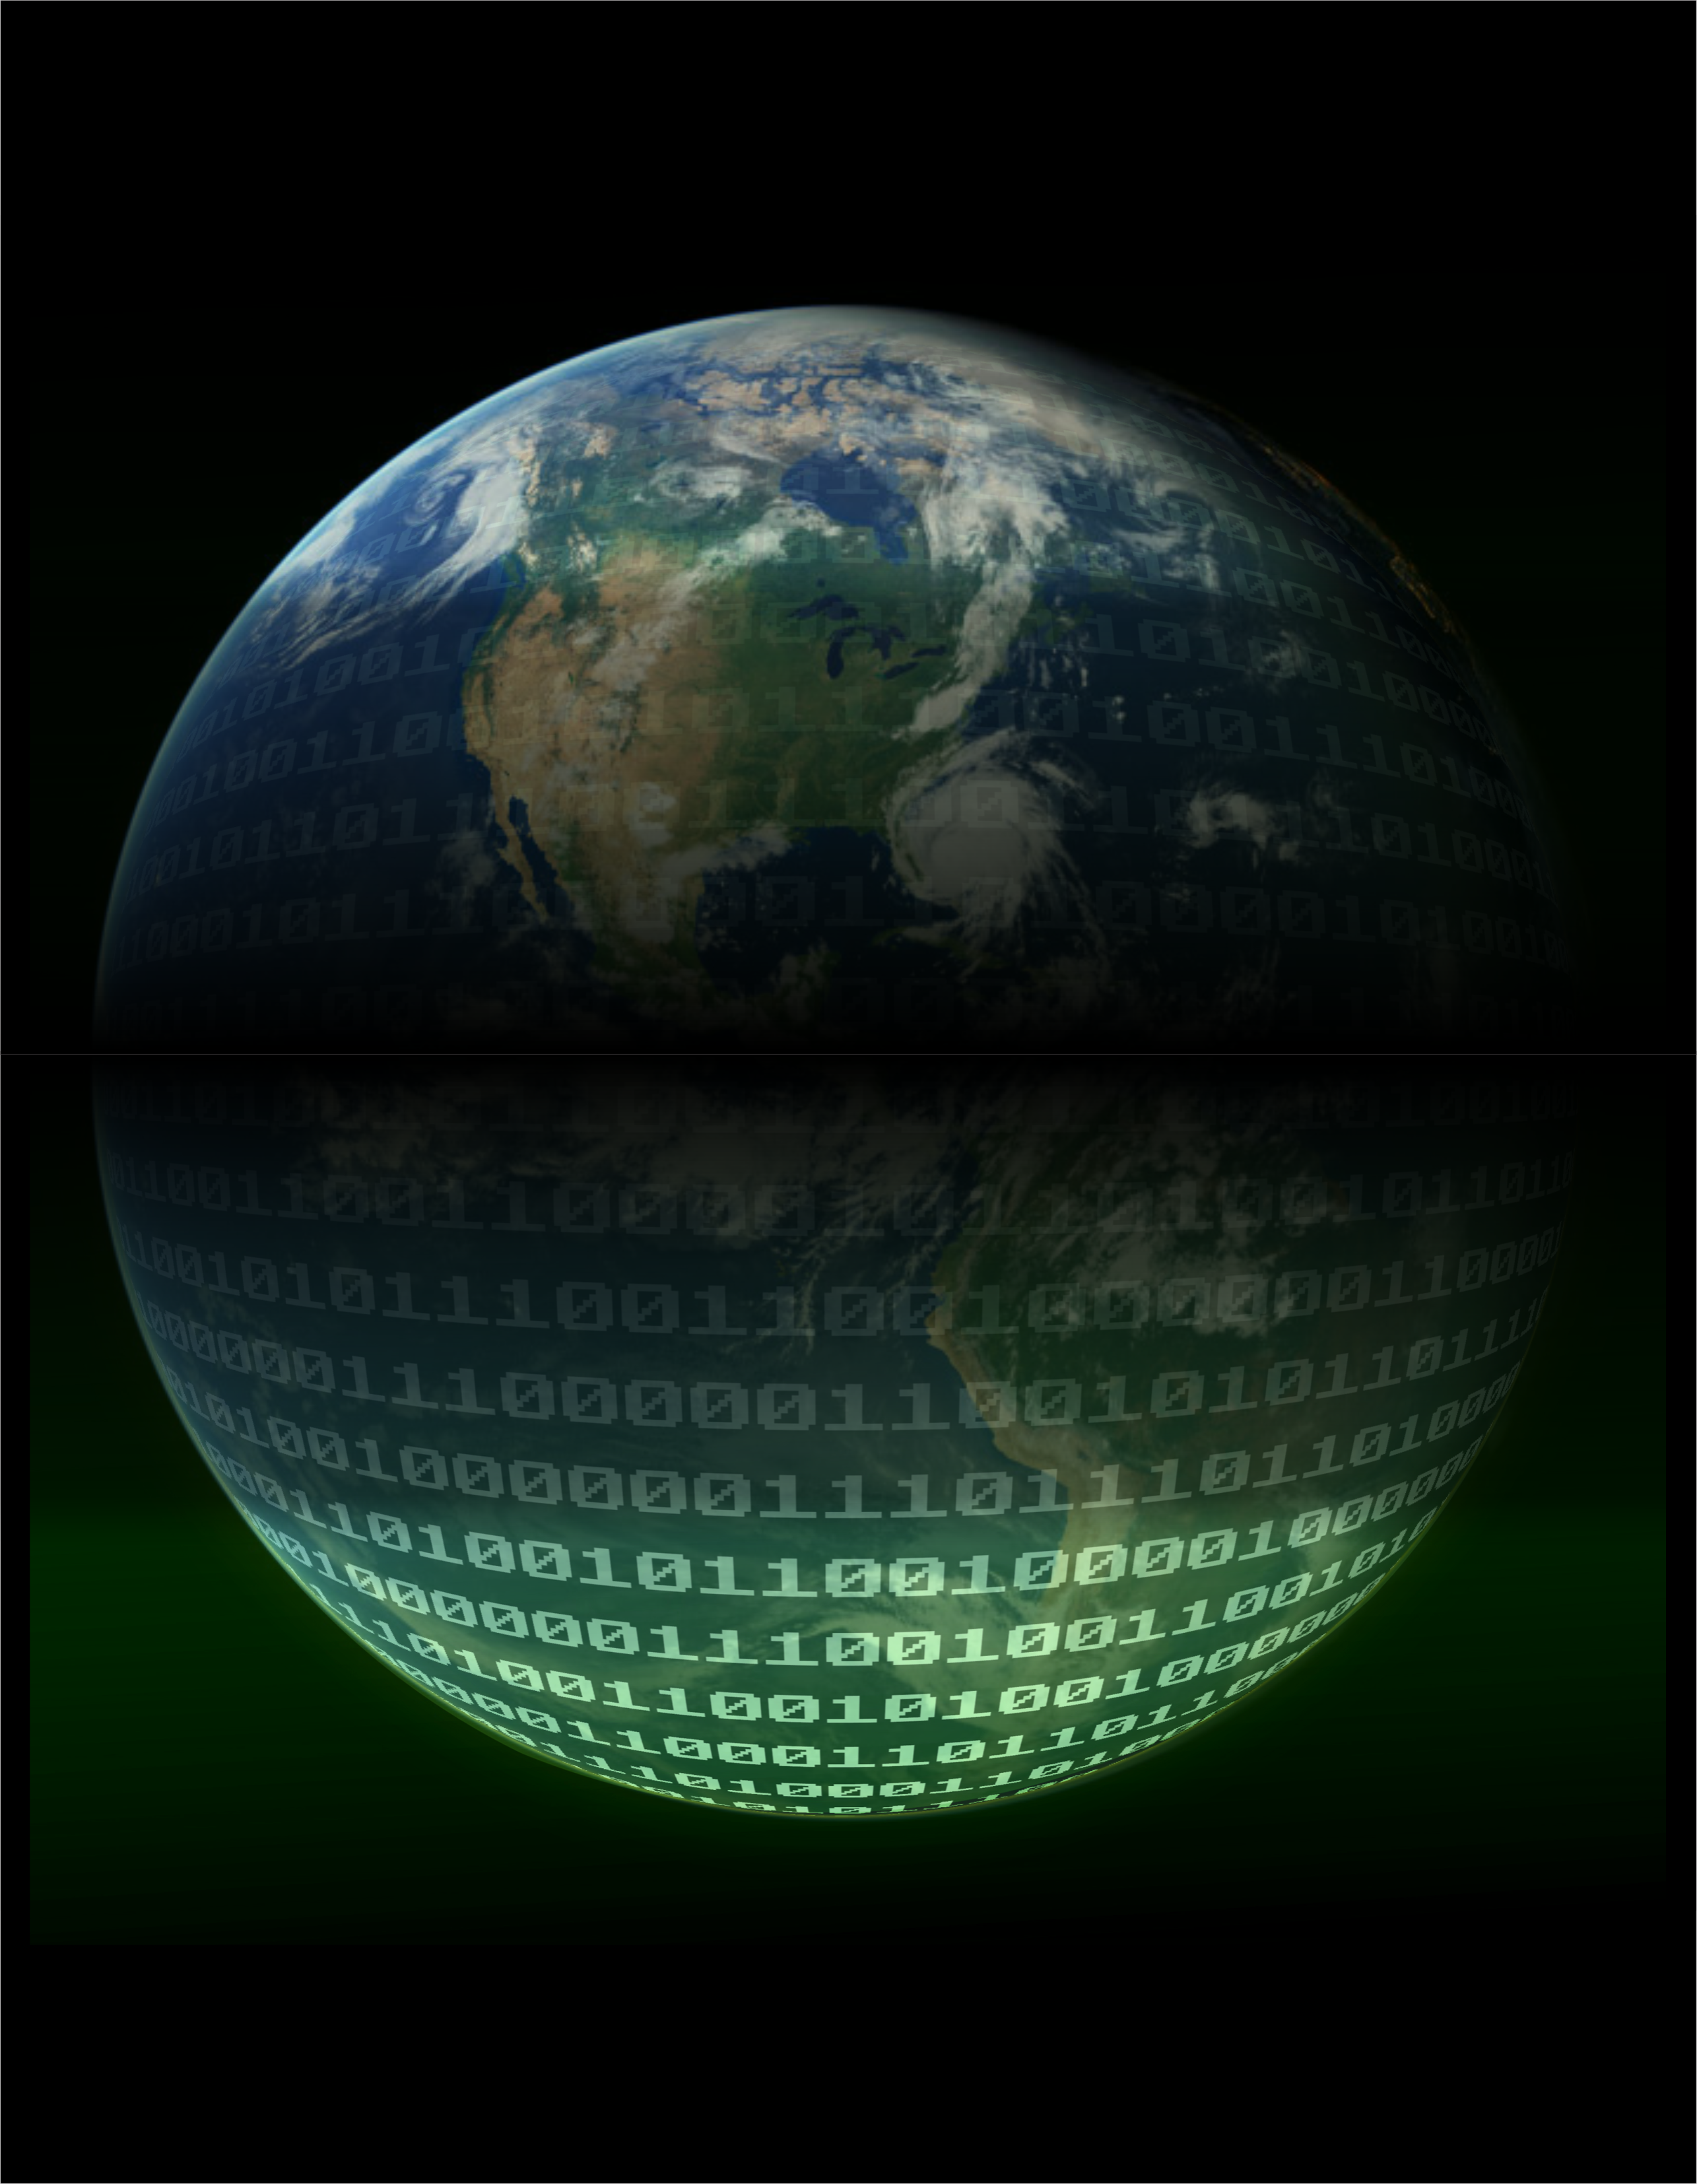
\includegraphics[scale=1.0]{cover}}} % Image background
\centering
\vspace*{7.5 cm}
\par\normalfont\fontsize{30}{30}\sffamily\selectfont
\textcolor[rgb]{1,1,0}{The Bumper Book of \textit{.cookie}s}\par % title
\vspace*{0.5cm}
\par\normalfont\fontsize{21}{21}\sffamily\selectfont
\textcolor[rgb]{0,0,1}{(The \textit{c}GENIE.cookie user-manual and introduction to Earth system modelling)}\par % title2
\vspace*{1cm}
{\Huge \textcolor[rgb]{1,1,1}{Andy Ridgwell}}\par % Author name
\endgroup

~\vfill
\textcolor[rgb]{1,0,0}{\today}

%----------------------------------------------------------------------------------------
%       COPYRIGHT PAGE
%----------------------------------------------------------------------------------------

\newpage
~\vfill
\thispagestyle{empty}

\noindent Copyright \copyright\ 2017 Andy Ridgwell\\ % Copyright notice

\noindent \textsc{Published by Derpy-cookies INC.}\\ % Publisher

\noindent \textsc{mycookie.seao2.org}\\ % URL

\noindent Licensed under the Creative Commons Attribution-NonCommercial 3.0 Unported License (the ``License''). You may not use this file except in compliance with the License. You may obtain a copy of the License at \url{http://creativecommons.org/licenses/by-nc/3.0}. Unless required by applicable law or agreed to in writing, software distributed under the License is distributed on an \textsc{``as is'' basis, without warranties or conditions of any kind}, either express or implied. See the License for the specific language governing permissions and limitations under the License.\\ % License information

\noindent \textit{First printing, October 2017} % Printing/edition date

%----------------------------------------------------------------------------------------
%       TABLE OF CONTENTS
%----------------------------------------------------------------------------------------

\chapterimage{courseimages.png} % Table of contents heading image

\pagestyle{empty} % No headers

\tableofcontents % Print the table of contents itself

\cleardoublepage % Forces the first chapter to start on an odd page so it's on the right

\pagestyle{fancy} % Print headers again

\mainmatter

%----------------------------------------------------------------------------------------
%----------------------------------------------------------------------------------------

%----------------------------------------------------------------------------------------
%----------------------------------------------------------------------------------------
%       CHAPTER 00
%----------------------------------------------------------------------------------------
%----------------------------------------------------------------------------------------

\cleardoublepage

\chapterimage{muffin_planet.jpg} % Chapter heading image

\setcounter{chapter}{-1}
\chapter{Installation, Configuration, Basic Usage}\label{ch:0}

\hfill \break

\vspace{16mm}

\noindent Stuff to keep in mind:

\vspace{2mm}

\begin{itemize}
\item \textbf{(cGENIE.)cookie} is a \uline{model}. Models ARE NOT the ‘real World’. (Don’t get confused!)
\item The  low resolution (for a 3-D ocean circulation model) of the \textbf{cookie} model limits its applicability for very short time-scale problems.\ In configurations not incorporating the \textbf{PLASIM} atmospheric GCM component, there are no atmospheric dynamics or inter-annual variability in the coupled ocean-atmosphere system.
\item \textbf{cookie} is best thought of as a ‘discovery and exploring’ tool for learning how the Earth system has functioned in the past rather than a detailed ‘simulation’ tool for the future.
\item It is possible to have fun.
\end{itemize}

%------------------------------------------------
\newpage
%------------------------------------------------

\section{Before anything else …}

%------------------------------------------------

\subsection*{ReadMe}

Some warnings and reminders in this manual are repeated over and over and over and … over again.
Some warnings and reminders are repeated over and over and over and … over again.
This is because you will forget immediately each time! ;)
\\\textbf{!}\footnote{\textbf{Also read footnotes please.}}

%------------------------------------------------

\subsection*{Software version naming conventions}

You will be using the current version of the cGENIE Earth system model, code-named ‘\textbf{cookie}’ (if \textbf{Apple} can have ‘Leopard’, ‘Lion’ etc., I can have a baked goods version naming convention). The documentation may not be fully consistent in this respect … and you may need to translate occurrences of e.g. a directory named ‘\texttt{cgenie}’ to ‘\texttt{cgenie.cookie}’. For brevity, the \textbf{cGENIE.cookie} model will be referenced by just ‘\textbf{cookie}’.

%------------------------------------------------

\subsection*{linux ...}

The \textbf{(cGENIE.)cookie} model currently naively compiles and runs under \textbf{linux}\footnote{For some of you, the mechanics of running the model will be about as much fun as sticking your tongue in an electrical outlet (a popular hobby in England). (However, if you are an experienced linux/unix/tongue-in-electrical-socket user, you can skip onto the next Section and save yourself an entire 15 seconds of reading words.)} (e.g. distributions such as \textbf{Ubuntu}) and unix-like operating systems (such as \textbf{macOS}). \textbf{cookie} (like most climate models) is configured and accessed (aka ‘run') at the ‘command line’ of the linux (or \textbf{macOS} equivalent, which is unix-like) operating system. The command line is a place where you type text and when you press \small\textsf{Return}\normalsize, something (hopefully, good!) happens. Typically the stuff you type started with a ‘command’ word, and often followed by one or more options and parameters. The command word and any options / parameters MUST be separated by SPACEs.

The start of each line of the command line is indicated with something like: \texttt{\$}. The \texttt{\$} is called the ‘prompt’ and is ... prompting you to type some input (commands, Tweets, swear words, etc.). See – the computer is just sat there waiting for you to command it to go do something (stupid?). Typically, you will also be informed (reminded) of the user-name, computer name, and current directory, e.g.:

\vspace{-2mm}
\begin{verbatim}
[username@host ~]$
\end{verbatim}
\vspace{-2mm}

\noindent which is in this example is user ‘\texttt{username}’ (yours will be different!) on computer name ‘\texttt{host}’\footnote{Sprout the cat will eventually appear under ‘cat-of-the-day’ on my home-page if you press \textsf{F5} enough times – all my computing clusters are named after my cats …} and the current directory is the ‘home’ directory -- represented by the \texttt{\~} symbol. If, for example, you were instead currently in the \texttt{myfolder} directory, you would see at the command prompt something like:

\vspace{-2mm}
\begin{verbatim}
[username@host myfolder]$
\end{verbatim}
\vspace{-2mm}

If you are not or not very familiar with the linux/unix command line, such as how to navigate up and down the directory tree and to display the contents of the current directory you are in – for a brief summary of some basic/useful \textbf{linux} commands and usage -- see the linux HOW-TO Section towards the back of the book.

NOTE: BE VERY CAREFUL that spaces are not missed out when typing out example lines. Also be careful not to confuse the number one (\texttt{1}) for the letter 'el' (\texttt{l}). Mis-spelling/typing is generally the most likely reason for things not working.

NOTE-the-second: If you find yourself terminally bored typing in long long instructions lines, you may be tempted to simply copy-paste from the cookie manual PDF to the command line, This can work, but firstly be aware that trying to copy-paste multiple lines at once is doomed to failure -- copy-paste the first line and then following that add the second (or subsequent) line.
Also note that the inverted comma symbol in the PDF is not the same inverted comma symbol that linux is expecting ... You should also make liberal use of the up arrow key that bring back the previously entered command (keep pressing the key for progressively older commands). For instance, a mistake in a command line can be corrected by bringing back the offending line and using the left/right arrows to navigate through the characters and correct any mistake.

NOTE-the-third: In places, instructions may be given for specific programs and computer platforms and hence may differ slightly from the software reality in front of you. Use your judgement in translating such instructions. Many other alternative software choices exist for editing files or viewing results, as are other ways of configuring software and file editing/transferring methodologies. Do what suits you best – you can view such instructions where they occur, as  more representing an example methodology rather than a literal interpretation of the Constitution.

%------------------------------------------------

\subsection*{Required computer hardware/software}

For running \textbf{cupcake}, your options are:

\begin{enumerate}[noitemsep]

\vspace{1mm}
\item \textbf{Remotely}
\\To do this, you will need an account on a linux-based server or cluster. You can use any platform (\textbf{linux}, \textbf{macOS}, \textbf{Windoz}, as well as \textbf{iOS} and \textbf{Android} (which is based on \textbf{linux} in any case)) to connect to the cluster. You will need the following software on your local machine:
\vspace{1mm}
\begin{enumerate}[noitemsep]
\setlength{\itemindent}{.2in}
\item A terminal (‘shell’) window. This is no problem for \textbf{linux} and \textbf{Mac} users (you already have one built in). For \textbf{Windows}, either download a simple (and old) \textbf{SSH} client (ssh-client) from my website\footnote{http://www.seao2.info//cgenie/software/ssh-client.exe} or you can get hold of e.g. \textbf{PuTTY} (http://www.putty.org/).
\item A sftp (secure file transfer) client for convenience (i.e. dragging and dropping files between local and remote computers, and opening files directly on the remote computer cluster). If you have installed ssh-client (\textbf{Windows}, above) then a sftp client is already included as part of this software. If using \textbf{PuTTY} (\textbf{Windows}) you might try downloading \textbf{WinSCP} (http://winscp.net/eng/index.php). For \textbf{macOS}, you can connect to the server through the \textbf{Terminal}, but some sftp software for viewing/navigating server file structure include: \textbf{FileZilla} (recommended), \textbf{Cyberduck}, \textbf{TextWrangler}. For linux, maybe \textbf{FileZilla}.
\end{enumerate}

\vspace{1mm}
\item \textbf{Locally}
\\It is  possible to install and run the ‘\textbf{(cGENIE.)cookie}’ Earth system model either on a linux box (e.g. \textbf{Ubuntu}) or on a \textbf{Mac} \footnote{Sets of detailed installation instructions are available in the HOW-TO section of this manual.}\footnote{It is also possible to run \textbf{cookie} under \textbf{Windows}.}. At a minimum, you will need:
\vspace{1mm}
\begin{enumerate}[noitemsep]
\setlength{\itemindent}{.2in}
\item A FORTRAN (f90 and f77 combatable) compiler of some sort.
\\This may come with the operating system as standard, possibly \textbf{gfortran}.
\item A \textbf{git} client.
\\If not standard, this is relatively easy to add and install.
\item Compiled \textbf{netCDF} libraries (not so much fun ...).
\end{enumerate}
\vspace{1mm}
To edit files and visualize results, you will need some specific software. The exact software will depend on your operating system, but essential are:
\vspace{1mm}
\begin{enumerate}[noitemsep]
\setlength{\itemindent}{.2in}
\item A viewer for netCDF format spatial data. A \textbf{Java} viewer called \textbf{Panoply} is provided by NCAR for all platforms – http://www.giss.nasa.gov/tools/panoply/
(Note that you will need \textbf{Java} installed!) (Or alternatively: \textbf{MATLAB}, \textbf{python}, etc..)
\item  A simple text editor, except not the rubbish default \textbf{Windows} one – you need one that can display \textbf{unix} ASCII text without screwing it up. Options for \textbf{Windows} users are:
\textbf{notepad++} (https://notepad-plus-plus.org/)
\textbf{SciTE} (https://www.scintilla.org/SciTE.html)
(\textbf{linux} and \textbf{Mac} users need no special/different editor compared with your standard editor – everything will display just fine). You can also use \textbf{linux} command line based editors such as \textbf{vi}.
\end{enumerate}
\vspace{1mm}

\end{enumerate}
\vspace{1mm}

%------------------------------------------------

\subsection*{File editors ...}

You will need to edit text-based configuration files, possibly in installing and configuring \textbf{cookie}, but definitely in configuring model experiments. So now might be a good time to check that you can use the/an editor! (You will also be using the same editor to view some of the model output.)

You have two alternative options for editing and viewing text files, depending on whether you are a \textbf{unix} nerd with no life, or prefer anything to do with computers to be wrapped in cotton wool and covered with dollops of treacle.
EITHER: Use the linux \textbf{vi} (/\textbf{vim}) application (or similar e.g. \textbf{emacs}) if you are familiar with it. I think that this pretty much sucks as a text editor and life is far too short and brutal if you don't like this sort of thing … OR ... use a suitable linux-friendly text editor (NOT \textbf{Micro\$oft} \textbf{Notepad}) in conjunction with the \textbf{Secure File Transfer Client}. For example: \textbf{SciTE} (http://www.scintilla.org/SciTE.html) is suitable, or \textbf{Notepad++}.

If you fiddle about with the settings under Options/Preferences in the \textbf{WinSCP} program and apply a little common sense, it should be possible to configure things so that you can simply double-click on a file in the remote (right-hand) window panel and it will open like magic (almost)! Saving the file after editing) should then result in the file being saved back to the cluster. Or you can select Edit With (and then \textbf{SciTE}) from right-mouse-button-clicking on the filename. Or ... a crude but workable approach is to use an sftp client to drag the file to your local machine (assuming \textbf{cookie} is installed remotely), edit it there, and then drag it back again.\footnote{Note that care still has to be taken to avoid certain \textbf{Microsoft} text editing programs under \textbf{Windoz}.)}

%------------------------------------------------
\vspace{1mm}\noindent\rule{4cm}{0.5pt}\vspace{2mm}
%------------------------------------------------

%------------------------------------------------
\newpage
%------------------------------------------------

\subsection*{Model documentation in general}

This (the \textbf{cookie} manual), and additional documentation (of varying degrees of up-to-date-ness) can be found:

\vspace{1mm}
\begin{enumerate}[noitemsep]
\setlength{\itemindent}{.2in}
\item On \href{https://github.com/genie-model/cookiedoc}{GitHub}.
\\The \textbf{latex} source for the documentation lives here, allowing you to compile the most up-to-date PDF document. And ... make changes yourself and have them incorporated into the official documentation\footnote{First clone the \textbf{git} repository. Make changes. Commit them locally. Make a 'pull request' ...}.
\\However, note that you will have to compile the latex source yourself to create a PDF ...
\item On my \href{http://www.seao2.info/mymuffin.html}{website}.
\\Here you can find compiled PDF versions of the documentation ... but it could be a little out of date (the up-to-date latex sources lives on \textbf{GitHub}).
\end{enumerate}

%------------------------------------------------

\subsection*{This document in particular}

The instructions  may not be entirely bug-free -– use your judgment.

%------------------------------------------------

\subsection*{Go!}

OK – now we are ready to start …

%------------------------------------------------
\newpage
%------------------------------------------------

\section{Starting (dozing?) off …}

You are going to be installing the model from scratch – why? Why not? It will be a happy character-building experience for you ... trust me ...

%------------------------------------------------

\subsection{Logging in!}

In running \textbf{cookie} locally -- log into your \textbf{linux}/\textbf{macOS} box (and skip on to the next section)! \footnote{If you fail at this step, you'll have to take up box-modelling instead.}

\noindent Or ... and much more likely to be the case -- if you are running \textbf{cookie} \uline{remotely} (e.g. via a user account on a computing cluster or server), then log into the remote server or cluster account using a 'suitable terminal program'\footnote{It very much depends on what software you are using. Provided are instructions for some \uline{examples}, but only examples, and your reality may be rather different.}:

\begin{itemize}
\vspace{1mm}
\item If logging in via a \textbf{linux}/\textbf{macOS} box, open the terminal/shell window and simply SSH in\footnote{If your current directory looks something like this: \texttt{[username@clustername \(\sim\)]\$}
then you are probably already logged in! Otherwise, it will look like: \texttt{username@localcomputername:\(\sim\)\$}}, e.g.

\vspace{-1mm}
\begin{verbatim}
$ ssh username@clustername
\end{verbatim}
\vspace{-1mm}

where \texttt{clustername}, the cluster (or remote server) name(!) might, for example, be
\\\texttt{catname.ucr.edu}, and enter your  account password (and tell it whether or not you want this password stored, if asked).
\vspace{1mm}
\\\textbf{IMPORTANT!} -- When you type in a password in \textbf{linux}, NOTHING appears on the screen, not even \texttt{********} as in common on \textbf{Windoz}. As you type (the password), characters are being entered ... you just cannot see them. Don't panic -- just type in the password (even if you cannot see characters appearing) and hit \textsf{\scriptsize Enter}.

\vspace{1mm}
\item On a \textbf{Windoz} machine – first start the \textbf{WinSCP} program (an sftp file transfer client). Under \textsf{\footnotesize Host Name}, enter the remote server or cluster name (e.g. \texttt{catname.ucr.edu}):
\\The \textsf{\footnotesize Port number} should be set to \textsf{\footnotesize 22} (except for \texttt{sterling.ucr.edu}). Enter your computing cluster user-name on the line below this (‘\textsf{\footnotesize User Name}’) and then the \textsf{\footnotesize Password}. Click on \textsf{\footnotesize Login}.
\\You will also need a terminal window. This can be opened by clicking on the ‘\textsf{\footnotesize Open session in PuTTY}’ icon on the top icon row, or pressing \textsf{\footnotesize Ctrl+P}. \\You should now have TWO windows open – a ‘shell’ window (lines of text on an otherwise blank screen) and a file manager (transfer) window. Ensure that you have both these before moving on. It is recommended that you maximize both these windows to full screen. (But no-one will die horribly for not doing so. Probably ...).
\\ You can also log in directly from the shell/terminal window e.g. \textbf{PuTTY} first (rather than first opening an sftp connection first).
 You will sill have to open an sftp connection for file transfer.
\end{itemize}

\vspace{1mm}
Note that the cluster you access may not use the standard 'port' number of \textsf{\footnotesize 22}. If your computer uses a different port number -- in the login window of your sftp client, simply change the number in the \textsf{\footnotesize Port} box, or if you are using the command line, you will need to type:
\vspace{-1mm}
\begin{verbatim}
$ ssh -p xxxxx username@clustername
\end{verbatim}
\vspace{-1mm}
where \textsf{\footnotesize xxxxx} is the port number.

%------------------------------------------------

\subsection{Downloading/installing the model code}

The next step is to download/install a copy of the source code for \textbf{cookie}. The current release of the \textbf{cGENIE} model (\textbf{cookie}) lives here:

\vspace{1mm}
\href{https://github.com/genie-model/cgenie.cookie}{\texttt{https://github.com/genie-model/cgenie.cookie}}
\vspace{2mm}

There are 2 options:

\begin{enumerate}

\vspace{1mm}
\item '\textbf{cloning}'
\\The \uline{preferred/advised} way is to \textit{clone} the repository to where you intend to run \textbf{cookie}\footnote{But see later for other/better ways of working.}. While you can also use a GUI based git client, easiest is at the command line (e.g. from your HOME directory), using the command \texttt{git clone}\footnote{This: "... clones a repository into a newly created directory, creates remote-tracking branches for each branch in the cloned repository, and creates and checks out an initial branch that is forked from the cloned repository’s currently active branch."}:
\vspace{-1mm}
\begin{verbatim}
$ git clone https://github.com/genie-model/cgenie.cookie.git
\end{verbatim}
\vspace{-1mm}

By doing this, you have created your own code repository (and an identical copy of the one hosted on GitHub). As part of the \texttt{git clone} command, you also automatically \textit{check out} (from your very own personal repository) a copy of the code. \footnote{Note that the major difference then with the \textbf{svn} system, is that previously, the GENIE code repository existed only on the University of Bristol server, and you \textit{checked out} the code remotely from there.}

\vspace{1mm}
\item Simple downloading.
\\\uline{Less good}, but OK if you simply want a copy of the code to run an experiment just once, or simply only want to see the code.) By downloading an archive file, containing all the code etc. For this -- click on the \textcolor[rgb]{0,0.501961,0}{green} \textsf{\footnotesize Clone or Download} button on \textbf{GitHub}, and select \textsf{\footnotesize Download ZIP}. You then unpack/unzip the files and directory structure where you want it. This [archive download] is a perfectly workable way to proceed ... as long as you neither want to update the code with whatever new developments or bug fixes occur in the future, nor want to have any code changes you might make, become part of the official \textbf{cookie} code  (i.e. it becomes a one-off installation that has no connection to the \textbf{GitHub} repository.

\end{enumerate}

%------------------------------------------------

\subsection{Configuring the code}

\noindent You may ... or may not, need to configure some local environment settings so that all the libraries etc. that are needed to compile \textbf{cookie} can be found. To a very limited extent, cookie will try and identify your computer and make the required setting automatically. The changes, if any, that you need to make will depend on the platform where you will be running \textbf{cookie} (i.e. the computer where you have just cloned (or downloaded) the code repository to). The currently recognized platforms and required actions are as follows:

\vspace{1mm}
\noindent The required configuration settings for \textbf{cookie} depend on the specific computing platform that you are running on. What follows is a list of the changes associated with some possible platforms that you might be using -- \uline{find the list name (\textbf{bold}) that corresponds to the platform that you are using} and ignore all the other options.\footnote{If you are using a platform not listed here, you may be able to simply adapt the instructions for one of the ones listed.}

%------------------------------------------------
\newpage
%------------------------------------------------

\begin{itemize}

\vspace{1mm}
\item \textbf{Ubuntu} -- no changes are necessary (with caveats).
\\ This is the default assumed platform. No changes are necessary IF the \textbf{netCDF} libraries are installed in their default locations and a relatively recent version of \textbf{netCDF} is used.\footnote{By 'relatively recent' -- the default settings assume that the \textbf{FORTRAN} and \textbf{C} \textbf{netCDF} libraries are separate.}

\vspace{1mm}
\item \textbf{sterling} (UCR cluster) -- no changes are necessary (the cluster is automatically identified).

\vspace{1mm}
\item \textbf{eevee} (UCR cluster) -- no changes are necessary (the cluster is automatically identified).

\vspace{1mm}
\item \textbf{macOS}
\\ Please refer to the separate \textbf{macOS} instructions.

\vspace{1mm}
\item \textbf{Windows} 
\\ Please refer to the separate \textbf{Windoz} instructions.

\vspace{1mm} 
\item \textbf{Otherwise} ...
\\... one or more edits will be required to the file \textsf{\footnotesize user.mak}, which lives in the \textsf{\footnotesize genie-main} directory.

\begin{enumerate}[noitemsep]
\vspace{2mm}
\item At the end of the \textsf{\footnotesize user.mak}, the \textbf{netCDF} path needs to be changed.
\vspace{1mm}  
\\First comment out\footnote{To 'comment out' a line -- simply add a \texttt{\#} symbol to the very start of the line. When \textbf{cookie} runs, this line will be ignored.}. i.e.,
\small\begin{verbatim}
  ### DEFAULT ###
  NETCDF_DIR=/usr/local
\end{verbatim}\normalsize
to
\small\begin{verbatim}
  ### DEFAULT ###
  #NETCDF_DIR=/usr/local
\end{verbatim}\normalsize
Then un-comment\footnote{To 'un-comment' a line -- simply remove (delete) the \texttt{\#} symbol from the beginning of the line.} the line: \texttt{\#NETCDF\_DIR=my\_path}
\\\uline{AND} change \texttt{my\_path} to be the path to your \textbf{netCDF} libraries ... the trick step :o)

\vspace{2mm}
\item For MacOS users, there are alternative machine type options depending on your CPU. You need to comment out \texttt{MACHINE=LINUX} in  \textsf{\footnotesize user.mak} and then chose and un-comment one of the following:
\small\begin{verbatim}
#MACHINE=OSX	# Intel processor
#MACHINE=OSX_M	# Apple silicon (M1, M2 etc.)
\end{verbatim}\normalsize

\end{enumerate}

\end{itemize}

%------------------------------------------------
\vspace{1mm}\noindent\rule{4cm}{0.5pt}\vspace{2mm}
%------------------------------------------------

\noindent If your computer is configured to use python v.2 by default and/or does not have python v.3, then you will need to make a few minor changes (see HOW-TO).

%------------------------------------------------
\newpage
%------------------------------------------------

\subsection{Testing the model code}

\noindent Finally, you need to test the code to ensure that all the files have been cloned/installed correctly.

\vspace{1mm} 
\noindent First, change directory (see: Figure \ref{fig:directories}, and refer to the linux HOW-TO) to\footnote{Note: the model is *always* run from \texttt{cgenie.cookie/genie-main}}:
\vspace{-2mm}\begin{verbatim}
cgenie.cookie/genie-main
\end{verbatim}\vspace{-2mm}

\noindent If you are not ‘linux-friendly’ (see: Section \ref{how-to-linux} for \textbf{linux} basics) – maybe at first do this in steps – list the contents of the directory (\texttt{ls}) to check where you are (i.e. what directories are available to chance to), then change to \texttt{cgenie.cookie} (\texttt{cd cgenie.cookie}), then list again (\texttt{ls}) (and see what further directories are there), then change to \texttt{genie-main} (\texttt{cd genie-main}), and only then … type\footnote{Remembering that the \texttt{\$} is to indicate the command line, and you do not actually type it in.}:
\vspace{-2mm}\begin{verbatim}
$ make testbiogem
\end{verbatim}\vspace{-2mm}

\noindent This compiles a basic carbon cycle enabled configuration of \textbf{cookie} and runs a short test, comparing the results against those of a pre-run experiment (also downloaded alongside the model source code). It serves to check that you have the software environment correctly configured. There may be some ’Warnings’ reported (== somepony’s sloppy programming) but these are not detrimental to the ultimate science results (we hope!).
\vspace{1mm}
If you see the error message:
\vspace{-2mm}\begin{verbatim}
make: *** No rule to make target 
\end{verbatim}\vspace{-2mm}
when you try this, you are probably in the wrong directory (it should be \textsf{\footnotesize cgenie.cookie/genie-main}).

%------------------------------------------------
\vspace{1mm}\noindent\rule{4cm}{0.5pt}\vspace{2mm}
%------------------------------------------------

\noindent ‘Success’ of this test is indicated by the message:
\vspace{-1mm}
\small\begin{verbatim}
**TEST OK**
\end{verbatim}\normalsize
\vspace{-1mm}

\noindent If you see this -- you can then be certain that the model you have installed is producing identical (within tolerance) results to everyone else in the World who has ever installed \textbf{cookie}. Note that the model will pause for a l o o o o n g time at the line:
\vspace{-2mm}
\small\begin{verbatim}
./genie.job -t -k -f configs/eb_go_gs_ac_bg_test.xml -o /home/genie00/cgenie_output
   -c /home/genie00/cgenie -g ../../cgenie -m "" > testbiogem.out;
\end{verbatim}\normalsize
\vspace{-2mm}

\noindent This is quite ‘normal’ – the model is thinking! Also -- ignore the compiler warnings … 

\vspace{1mm}
\noindent \uline{This completes the basic code installation.}

\vspace{1mm}
\noindent If the test doesn't 'work'\footnote{Note that if you have disabled the compilation of the C program that compares netCDf files, the test will run but never complete and you'll not get a \texttt{**TEST OK**} reported, even if the test experiment ran correctly.} -- try issuing the command:
\vspace{-2mm}\begin{verbatim}
$ make cleanall
\end{verbatim}\vspace{-2mm}

\noindent and then re-try the test. 

\vspace{1mm}
Refer to the FAQ section at the end of this book for further clues as why the model installation appears not to be working.

%------------------------------------------------
\newpage
%------------------------------------------------

\noindent Note that \textbf{GitHub} does not host files larger than 100 MB, and the 'lookup table' for calculating opal dissolution in sediments (see e.g., \textit{Ridgwell et al.} [2003]) is larger than this. It has hence been committed to \textbf{git} as an archived file. \uline{Only if} a silica cycle is to be employed in your \textbf{cookie} experiments, does this file need to be unpacked. A script is provided for this -- from \texttt{genie-main}, type:

\vspace{-2mm}
\begin{verbatim}
$ ./installcookie.sh
\end{verbatim}
\vspace{-2mm}

\noindent and this will unpack the opal lookup table to \texttt{genie-sedgem/data/input} as well as unpacking a copy of the calcium carbonate lookup table\footnote{For now, the \(CaCO_{3}\) lookup table also included in the git repo in its expended (unpacked) form.}.

%------------------------------------------------
\vspace{1mm}\noindent\rule{4cm}{0.5pt}\vspace{2mm}
%------------------------------------------------

\subsubsection*{Some brief notes on git}

The simplest workable installation of \textbf{cookie}, as described above, is to use \texttt{git clone}. You end up with a carbon copy of the cookie code repo (I am too lazy to type out 'repository' again) which you have also automatically now 'checked out'. Changes and developments will occur to the code on the GitHub repo from time-to-time, and if may be that either you might benefit by using a more up-to-date code base, or specific changes may have been made that you absolutely need. To determine the status of your repo, type\footnote{Here, the -uno ensures that files (e.g. experiment configuration files) you have created, but not added and committed, are not listed.} (from \texttt{cgenie.cookie}):

\vspace{-2mm}
\begin{verbatim}
$ git status -uno
\end{verbatim}
\vspace{-2mm}

\noindent However, git has not actually compared your repo with the one on GitHub, because this is apparently network expensive (as if you don't spend the rest of your life killing the internet by streaming Rick and Morty). So, use:

\vspace{-2mm}
\begin{verbatim}
$ git fetch
\end{verbatim}
\vspace{-2mm}

\noindent which will 'download [new and modified] remote content but not update your local repo's working state'. If you now type \texttt{git status -uno}, \textbf{git} can tell you if there is newer content (e.g. '\texttt{Your branch is behind 'origin/master}'\footnote{\texttt{origin} is the origin of the repo -- GitHub, and \texttt{master} is the name of the branch, in this case, the default branch name.}). To merge in the fetched content:

\vspace{-2mm}
\begin{verbatim}
$ git merge
\end{verbatim}
\vspace{-2mm}

Both these commands are also combined in a single command\footnote{If there are no changes (to \textit{fetch} and \textit{merge}), the you get the message: \texttt{Already up-to-date.}}:

\vspace{-2mm}
\begin{verbatim}
$ git pull
\end{verbatim}
\vspace{-2mm}

If you are not developing code, and hence not editing files in the repo (but e.g. only adding new model configuration files), your life should mostly be trouble-free with regards to updating your code via \texttt{pull}.\footnote{
One exception is, if any of the model installation/configuration files that you might have edited, i.e. one or all of: \texttt{genie-main/user.mak}, \texttt{genie-main/makefile.arc}, and/or \texttt{genie-main/makefile}, have also changed on \texttt{origin/master}, then \texttt{pull} (or \texttt{merge}, after \texttt{fetch}) will fail (with the message: '\texttt{Please, commit your changes or stash them before you can merge. Aborting}'). The root issue is a conflict between remote file changes, and local ones that you had not committed to your repo.

You probably want to keep your local configuration changes, otherwise you'll probably end up re-doing them all over again. One solution is to sneakily 'hide' (\textit{stash}) them out of sight, by:
\$ git stash
\noindent You can now pull, updating your repo with respect to \texttt{origin/master}. Then -- you want your changes back, so apply the stashed changes:
\$ git stash apply
If unlucky, there will be conflict as your stashed changed are merged back onto your local repo branch (master). If so, you'll need to edit the file, deciding which line(s) is correct, and delete the version you do not want, along with the ASCII tags/labels.
}

%------------------------------------------------

\begin{figure}
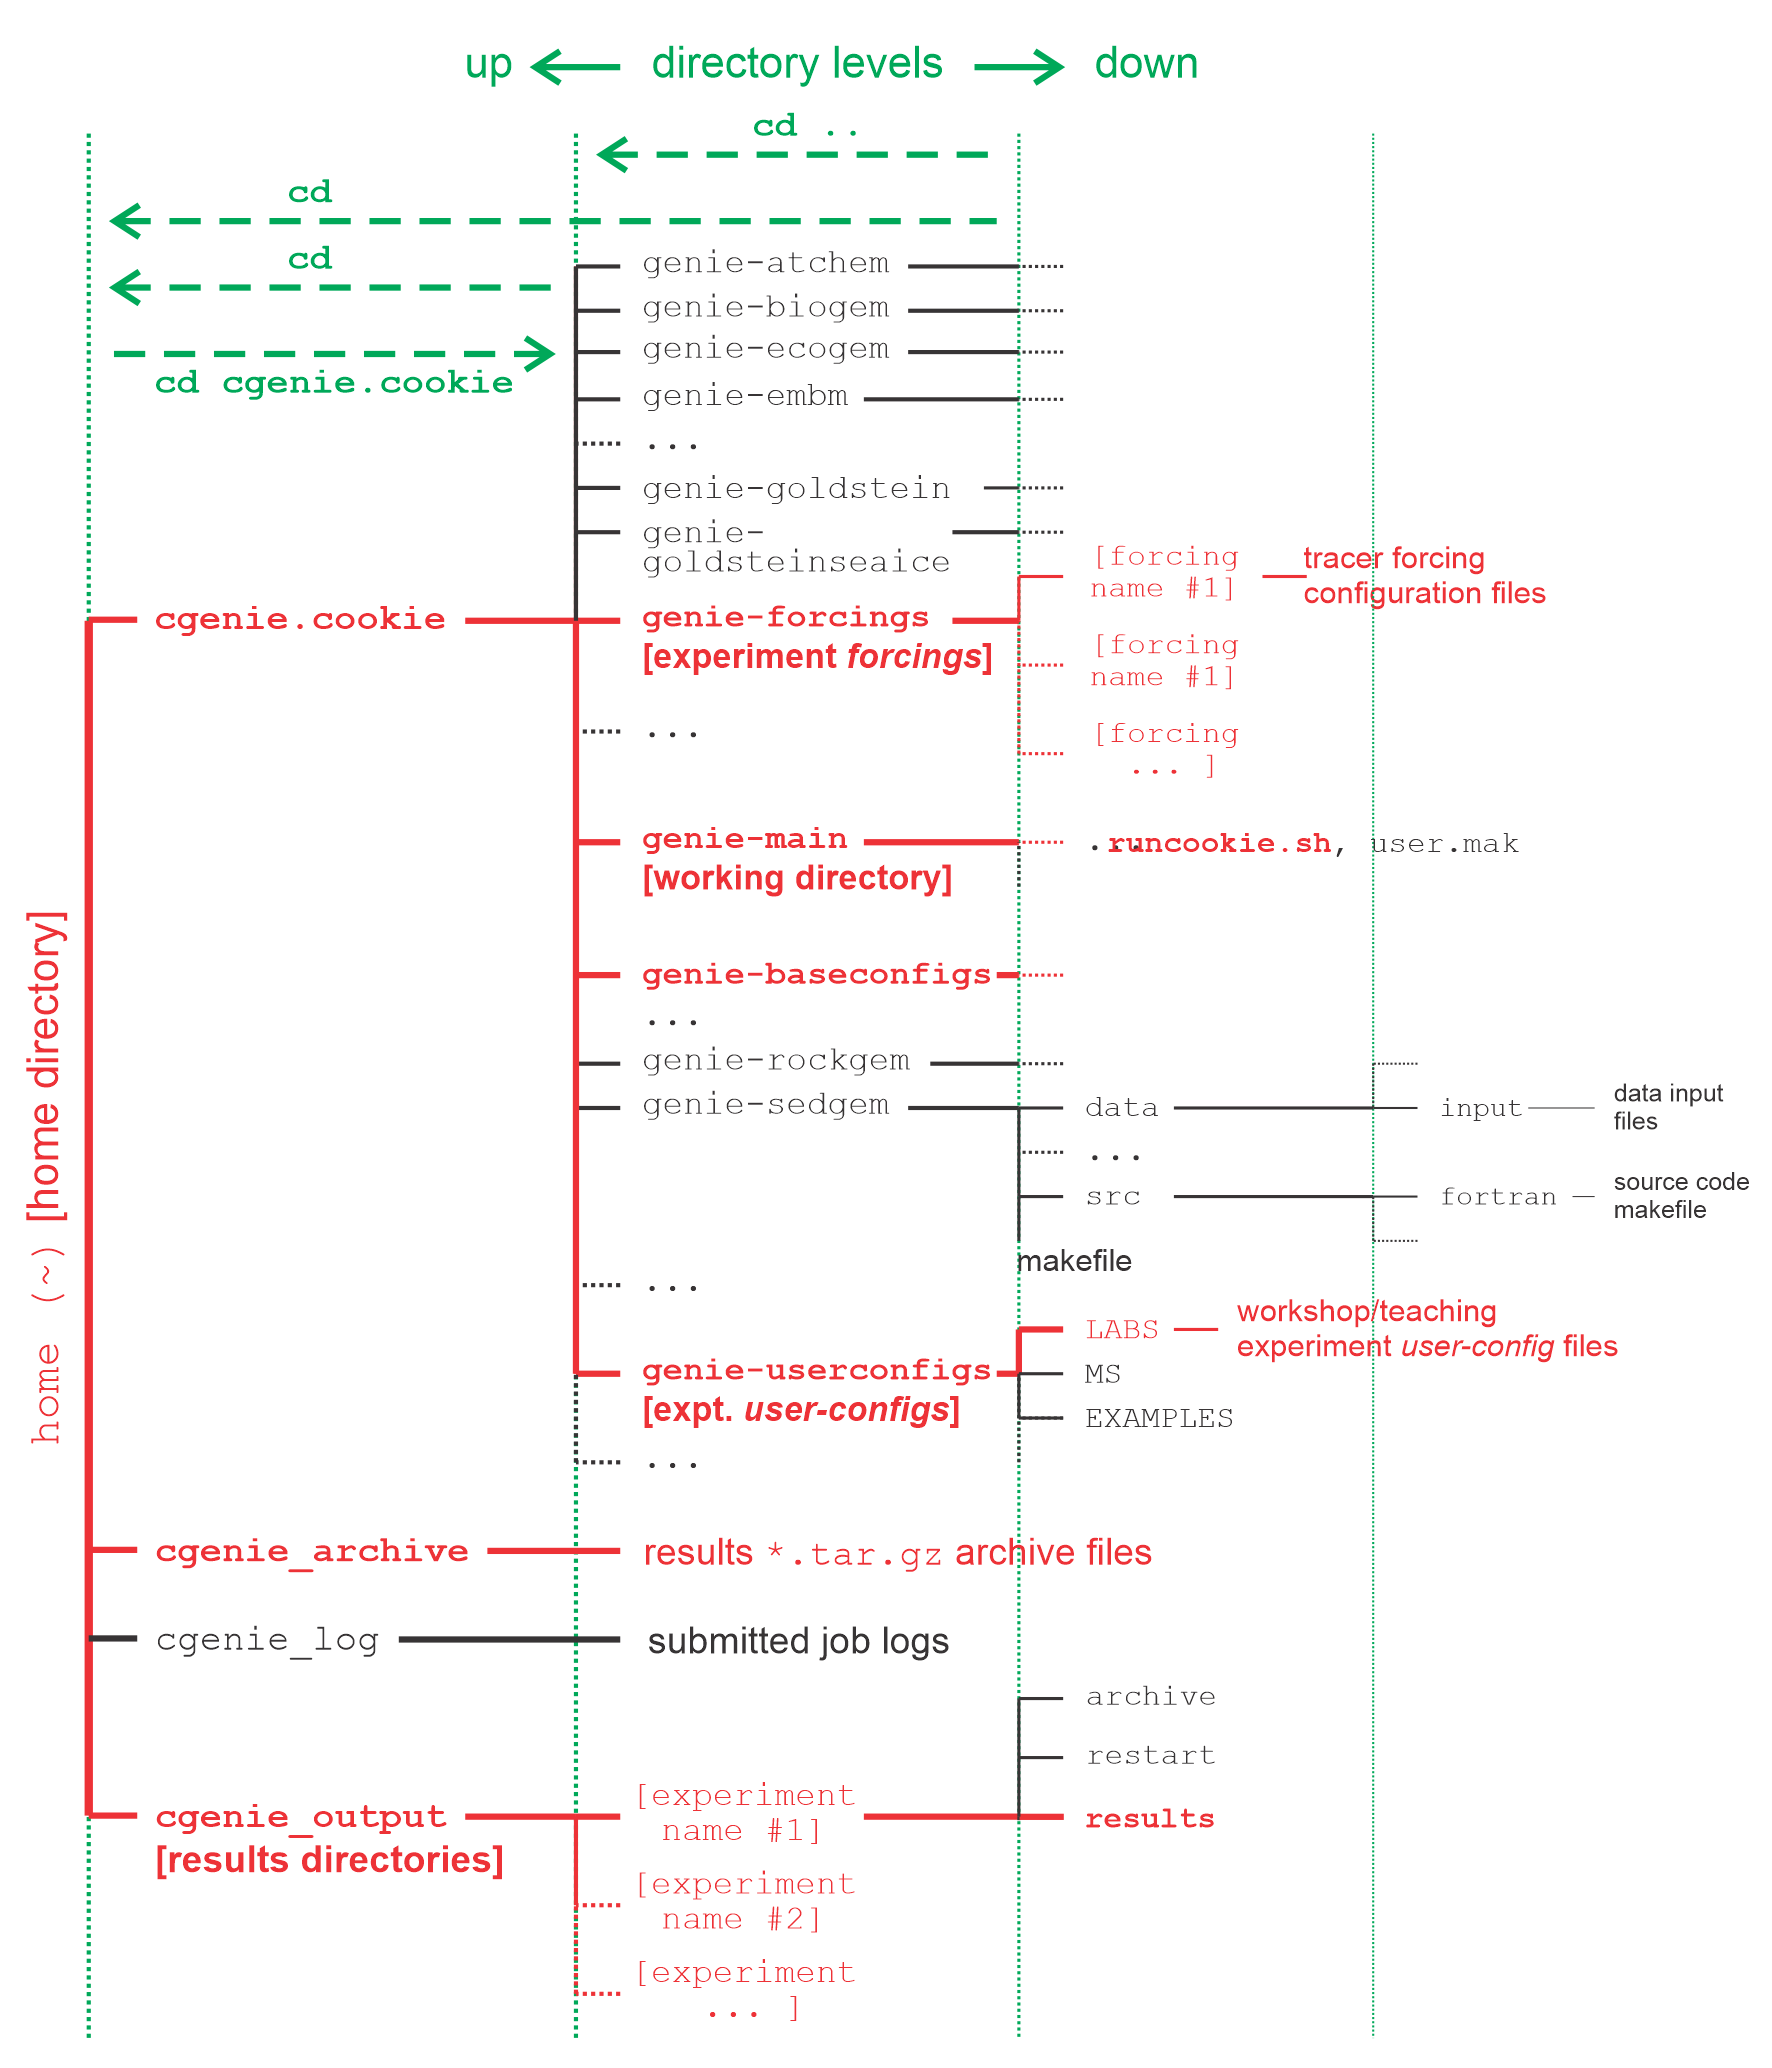
\includegraphics[width=\linewidth]{Figures.usermanual.1.png}
\caption{Directory structure of the \textbf{cookie} model. Highlighted in \textcolor{red}{red} are directories and sub-directories that you will need to access at some point. Vertical \textcolor[rgb]{0,0.501961,0}{green} lines designate directory levels, with example commands shown for moving between them.}
\label{fig:directories}
\end{figure}

%------------------------------------------------
\newpage
%------------------------------------------------

\section{Running the model}

The overall sequence of configuring and running \textbf{cookie} (job submission to a cluster queue), is shown in Figure \ref{fig:chx-jobcreation}. Refer to this if in any doubt at any point.

At the command-line (\texttt{\$}) and \uline{in the \textsf{\footnotesize genie-main} directory} (not your home directory), you will be entering in a command (\texttt{./runcookie.sh}) together with a list of parameters that will be passed to the model, and as if by magic the model will run (or sometimes not). The form of the command you are going to be issuing is:

\vspace{-1mm}\begin{verbatim}
$ ./runcookie.sh #1 #2 #3 #4 (#5)
\end{verbatim}\vspace{-1mm}

\noindent(\uline{don't type it yet}!) It requires that you must list at least 4 parameters after \texttt{./runcookie.sh}, separated by S P A C E S and on a single continuous line (even if it ‘wraps’ around across 2 lines of the screen).
These parameters are:

\vspace{2mm}
\begin{enumerate}[noitemsep]
\setlength{\itemindent}{.2in}
\item[\textbf{\#1}] ... is the name of the required base (or ‘basic’) configuration (‘\textit{base-config}’) of the model.
\item[\textbf{\#2}] ... is the name of the subdirectory (if any) containing the user configuration (‘\textit{user-config}’) file (i.e., the file containing the specification of a particular experiment).
\item[\textbf{\#3}] ... is the name of the experiment itself. There must exist a file in the directory specified by parameter \#2 (\texttt{LABS}) with exactly the same name as you enter here for parameter \#3 (i.e. parameter \#3 points to a file in the directory given by parameter \#2).
\item[\textbf{\#4}] ... is the run length of the experiment in years – this must be entered as an integer.
\item[\textbf{(\#5)}] ... There is also one optional (5th) parameter (to be described later).
\end{enumerate}

%------------------------------------------------
\vspace{1mm}\noindent\rule{4cm}{0.5pt}\vspace{2mm}
%------------------------------------------------

\noindent As an example of running the \textbf{cookie} Earth system model:

\vspace{2mm}
\begin{enumerate}[noitemsep]
\setlength{\itemindent}{.2in}
\item[\textbf{\#1}]: The \textit{base-config} is: \texttt{cookie.CB.p\_worbe2.BASES}
\item[\textbf{\#2}]: The \textit{user-config} directory is: \textsf{\small LABS}
\item[\textbf{\#3}]: The \textit{user-config} file (the experiment name) is: \texttt{LAB.0.3.EXAMPLE}.
\item[\textbf{\#4}]: Run the experiment for ten years: 10
\item[\textbf{\#5}]: (There is no restart file, and so no 5th parameter needs to be passed …)
\end{enumerate}

The full command for your first example experiment, which you are going to issue from the \texttt{\~}\texttt{/cgenie.cookie/genie-main} directory, then looks like:

\vspace{-1mm}\begin{verbatim}
$ ./runcookie.sh cookie.CB.p_worbe2.BASES LABS LAB.0.3.EXAMPLE 10
\end{verbatim}\vspace{-1mm}

\noindent(\uline{you can try it now}!)

\vspace{2mm}
\textbf{REMEMBER: This must be entered on a single CONTINUOUS LINE.}

\textbf{The (single) S P A C E S are vital. }

\textbf{ALSO -- take care not to confuse an el (‘\texttt{l}’) with a one (‘\texttt{1}’)  ... (it is a ‘one’ here).}

%------------------------------------------------
\newpage
%------------------------------------------------

\noindent What should happen is: First, you will end up twiddling your thumbs a while, as all the components of \textbf{cookie} are compiled from the raw source code (\textbf{FORTRAN}). When it has finished doing this, the model will initialize and carry out some brief self-checking. Only then will it start actually ‘running’ and doing something ... in this particular example, the output should look something like this:

\vspace{-2mm}\tiny\begin{verbatim}

 *******************************************************
  *** Initialisation complete: simulation starting ...
 *******************************************************

 >   model year |   pCO2(uatm)   SAT(oC) |   AMOC(Sv)    ice(%)   SST(oC)  SSS(PSU) |       pH  OHMEGA |   [O2](uM)  fPOC(PgC/yr)

 >          0.5 |      285.042    -3.667 |     12.715     0.274     1.408    34.902 |    8.048   2.537 |    181.360        12.327
 >          1.5 |      295.295    -2.531 |     13.189     2.126     3.450    34.902 |    8.079   2.896 |    191.671        12.636
 >          2.5 |      302.383    -1.270 |     12.266     4.282     5.004    34.904 |    8.088   3.131 |    196.879        12.394
 >          3.5 |      307.657    -0.274 |     11.020     5.525     6.214    34.906 |    8.093   3.318 |    199.930        12.216
 >          4.5 |      311.667     0.628 |      9.831     6.037     7.185    34.908 |    8.096   3.469 |    201.861        12.096
 >          5.5 |      314.811     1.437 |      8.876     6.387     7.987    34.910 |    8.099   3.597 |    203.157        11.994
 >          6.5 |      317.299     2.150 |      8.091     6.628     8.667    34.911 |    8.101   3.707 |    204.047        11.899
 >          7.5 |      319.290     2.782 |      7.872     6.673     9.256    34.913 |    8.103   3.800 |    204.669        11.822
 >          8.5 |      320.852     3.342 |      7.886     6.734     9.773    34.914 |    8.105   3.882 |    205.073        11.742
 >>> SAVING BIOGEM TIME-SLICE AVERAGE CENTERED @ year  :        9.500
 >          9.5 |      322.066     3.848 |      7.935     6.684    10.232    34.914 |    8.106   3.954 |    205.320        11.670

 *******************************************************
  *** Simulation complete: shutdown starting ...
 *******************************************************

\end{verbatim}\normalsize\vspace{-2mm}

%------------------------------------------------
\vspace{1mm}\noindent\rule{4cm}{0.5pt}\vspace{2mm}
%------------------------------------------------

\noindent What do all these numbers mean? From left-to-right:

\vspace{1mm}\begin{itemize}
\item[] \texttt{model year}  -- ... guess!
\end{itemize}\vspace{1mm}

\noindent Then:

\vspace{1mm}\begin{itemize}
\item[] p\(CO_{2}\)(uatm) -– mean atmospheric CO\(_{2}\) concentration (in units of \(\mu\)atm)
\item[] \texttt{<SST>} -- global mean surface air temperature ('SAT') $^{\circ}$C
\end{itemize}\vspace{1mm}

Note that if you are not running an experiment without a carbon cycle, there will be no values for p\(CO_{2}\).

\vspace{1mm}\begin{itemize}
\item[] \texttt{AMO(Sv)} -- Atlantic meridional overturning circulation (AMOC) (Sv)
\item[] \texttt{ice(\%)} -- global sea-ice fraction (\%)
\item[] \texttt{<SST>} -- global sea surface temperature ('SST') $^{\circ}$C
\item[] \texttt{<SSS>} -- global sea surface salinity ‘SSS’ (\%\textit{o})
\end{itemize}\vspace{1mm}

Note that if you are not running an experiment with a modern-like Atlantic basin, no value is given for the AMOC.

\noindent After that, a couple of carbonate chemistry indicators:

\vspace{1mm}\begin{itemize}
\item[] \texttt{pH} -- Mean ocean surface pH.
\item[] \texttt{OHMEGA} -- Mean ocean surface OHMEGA ...
\end{itemize}\vspace{1mm}

\noindent which will become apparent later.

Note that if you are not running an experiment without a carbon cycle, no values will be given.

\noindent Finally:

\vspace{1mm}\begin{itemize}
\item[] \texttt{O2} -- Dissolved oxygen in the ocean(global mean). ($\mu mol kg^{-1}$)
\item[] \texttt{fPOC} -- Global total annual export production (in terms of particulate organic carbon ($PgC yr^{-1}$).
\end{itemize}\vspace{1mm}

Note that you need some sort of biological pump in the ocean for these to be meaningful.

%------------------------------------------------
\vspace{1mm}\noindent\rule{4cm}{0.5pt}\vspace{2mm}
%------------------------------------------------

\noindent The choice of what information to display on screen as the model is running is rather arbitrary, but the chosen metrics do tend to summarize some of the main properties of the climate system and carbon cycle – for my own personal convenience rather than reflecting any fundamental scientific truth ... 

This information is reported at the same intervals as \textit{time-series} data (see later and/or refer to the User Manual) is saved and is indicated by:

Interleaved between these lines are lines reporting the saving of \textit{time-slice} data (the 2- and 3-D model states – more of which later as well as in the User Manual). These appear as:

\vspace{-2mm}\small\begin{verbatim}
>>> SAVING BIOGEM TIME-SLICE AVERAGE CENTERED @ year:
\end{verbatim}\normalsize\vspace{-2mm}

%------------------------------------------------
\vspace{1mm}\noindent\rule{4cm}{0.5pt}\vspace{2mm}
%------------------------------------------------

\noindent \textbf{You can stop the model at any point (all data up to that time will have been saved) by hitting: \textsf{\footnotesize <Ctrl-C>} (\textsf{\footnotesize CONTROL} key + ‘\textsf{\footnotesize C}’ key).}

%------------------------------------------------
\vspace{1mm}\noindent\rule{4cm}{0.5pt}\vspace{2mm}
%------------------------------------------------

\noindent Just from examining the screen output: how close to steady state does the system appear to have come after just 10 years? i.e., do SST and/or sea-ice extents appear to be converging towards stable (constant) values? This will be an important question to think about later on: ‘has the model reached steady-state (and does it matter)?’

%------------------------------------------------
\newpage
%------------------------------------------------

\begin{figure}
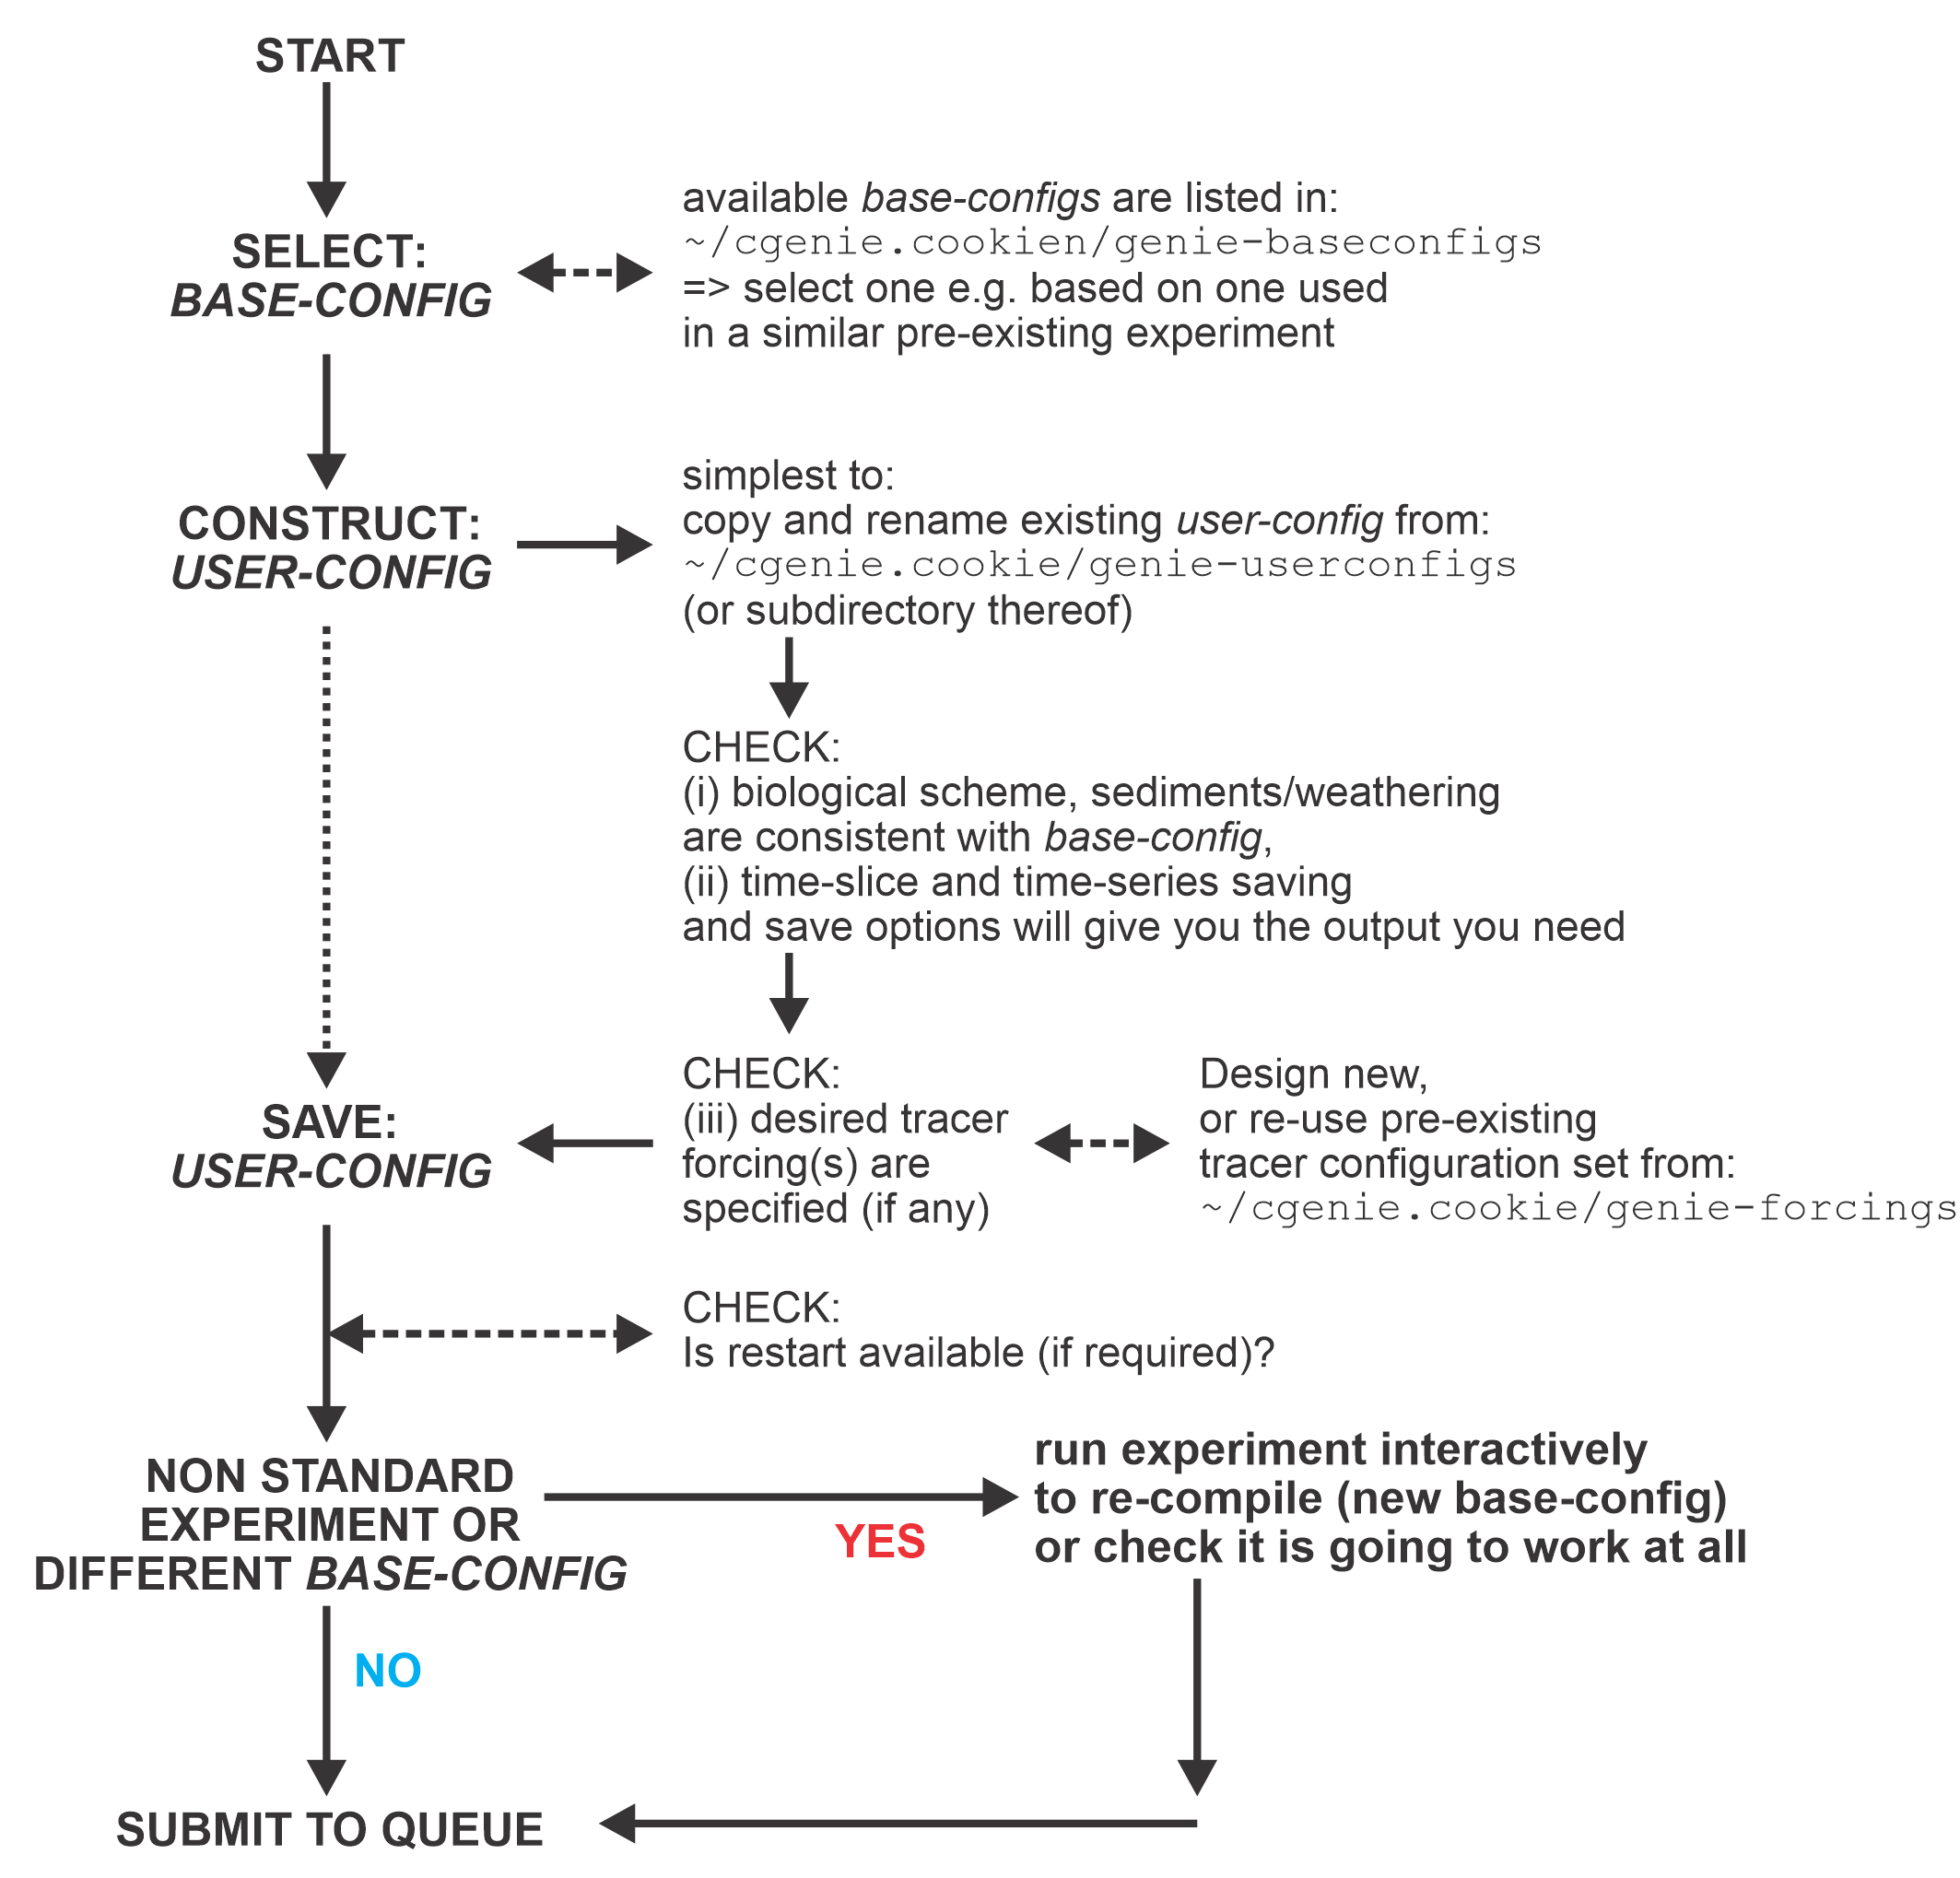
\includegraphics[width=0.9\textwidth]{Figures.usermanual.2.png}\centering
\vspace{2mm}
\caption{Schematic of the sequence-of-events in configuring and running an experiment.}
\label{fig:chx-jobcreation}
\end{figure}

%------------------------------------------------
\newpage
%------------------------------------------------

\section{Creating new experiments!}

The key to creating new experiments is to \textbf{remember that the name of the \textit{user-config} file, that contains the parameter settings that define that specific experiment, becomes the name of the experiment and hence name of the model results sub-directory in \textsf{\footnotesize cgenie\_output}}. Changing the name of the \textit{user-config} file, hence leads to a new experiment name and a new model results sub-directory. (Conversely, not changing the name of the  \textit{user-config} file and re-running it results in the results of any previous experiment run using that \textit{user-config} file, being over-written.)

%------------------------------------------------
\newpage
%------------------------------------------------

There are two obvious ways to create a new \textit{user-config} file and hence new experiment (although the simplest and recommended way, is the 2nd one):

\begin{enumerate}[noitemsep]

\vspace{1mm}
\item Create a blank text file \footnote{\texttt{\$ touch file.txt} will achieve this at the linux command line.} and populate the contents with the parameter value assignments you need for your new experiment.
\\Inevitably, it is difficult to remember all the names and even values you want to specify, meaning that you'll end up looking at existing \textit{user-config} files and copying and pasting lines (or even the entire contents) from the old file(s) into your new \textit{user-config} file. So then you may was well ...

\vspace{1mm}
\item Copy and edit an existing file!
\\This is the most practical approach -- pick an existing \textit{user-config} file that is closest to the specific experiment that you want to run -- copy and rename it, then edit the contents and save. For the purpose of trying this out, you can literally pick on any existing file in the \textsf{\footnotesize LABS } subdirectory (of \textsf{\footnotesize genie-userconfigs}).
\vspace{1mm}
\\ You can do this by:
\begin{itemize}[noitemsep]
\vspace{1mm}
\item Using your sftp client (program):
\\First -- drag the existing \textit{user-config} file to your local computer. On your local computer, rename the file as per how you would 'normally' rename any file. 
\\Now you can edit the parameter values, re-save it, drag it back to the cluster (from your local computer) using the sftp client ... and finally run the experiment.
\\There are also ways of configuring \textbf{sftp} clients so that you can double-click on a file in the remove window, edit it, and save it back to the remote computer.\footnote{Actually what happens is that the file is transferred locally, opened, and you edit a local copy. When you save it (locally), it is automatically transferred back.} 
\vspace{1mm}
\item Or, if you are comfortable working at the linux command line; working from the same directory (e.g. \textsf{\footnotesize LABS}) that the file you want to copy lives in, you can copy a file (to a new filename) by:
\\\texttt{\$ cp oldfile newfile }
\\(after which you can edit the new \textit{user-config} file \textsf{\footnotesize newfile}, re-save, and then run the experiment.)
\end{itemize}
\vspace{1mm}

\end{enumerate}

\noindent Remember that the new \textit{user-config} file needs to be saved in (or copied to) the \textsf{\footnotesize genie-userconfigs/LABS} sub-directory (in the case of experiments carried out as part of the tutorials described in this manual), or \textsf{\footnotesize LABS} itself or any sub-directory (or sub-sub- etc directory) ... as long as you specify the correct path to the directory where you save the new file to\footnote{See previous Section and the use of the 2nd parameter passed to \texttt{runcookie.sh}}.

%------------------------------------------------
\newpage
%------------------------------------------------

\section{Model output}

Experiment results are saved in a single sub-directory of the experiment results directory (along with a sub-directory for \textit{restart} files, and one for copies of your parameter choices). The experiment results directories all live in:

\vspace{-1mm}\begin{verbatim}
~/cgenie_output
\end{verbatim}\vspace{-1mm}
and will be assigned a directory name something like:

\vspace{-1mm}\begin{verbatim}
LAB.0.3.EXAMPLE
\end{verbatim}\vspace{-1mm}
(this being the results directory name for an experiment called \textsf{\footnotesize LAB.0.3.EXAMPLE}) and the actual results results hence in:

\vspace{-1mm}\begin{verbatim}
~/cgenie_output/LAB.0.3.EXAMPLE/results
\end{verbatim}\vspace{-1mm}

\noindent NOTE: If in an sftp client window you find that you cannot 'see' the \textsf{\footnotesize cgenie\_output} directory ... or cannot find any of the results sub-directories you are expecting, \uline{you will need to refresh the directory listing} (e.g. for \textbf{WinSCP}, there is a double green-arrow \textsf{\footnotesize Refresh} icon button near the top right of the window that you can click on). sftp client programs generally do not automatically refresh directory listing on the remote computer.

%------------------------------------------------
\vspace{1mm}\noindent\rule{4cm}{0.5pt}\vspace{2mm}
%------------------------------------------------

\noindent \textbf{cGENIE.cookie} has a flexible and powerful facility of saving results by means of spatially explicit ‘time-slices’, and as a semi-continuous ‘time-series’ of a single global (or otherwise representative mean) variable, described as follows.

%------------------------------------------------

\subsection{Time-slice output}

One of the most informative data sets that can be saved is that of the spatial distribution of properties (such as tracers or physical ocean attributes). However, saving full spatial distributions (e.g., a 36\(\times\)36\(\times\)8 array) for any or all of the tracers each and every time-step is clearly not practical; not only in terms of data storage but also because of the detrimental effect that repeated file access has on model run-time.
Instead, \textbf{BIOGEM} will save the full spatial distribution of tracer properties only at one or more predefined time points (in units of years). These are termed \textit{time-slices}. At the specified time points, a set of spatially-explicit data fields are saved for all the key tracer, flux, and physical characteristics of the system. However, rather than taking an instantaneous snapshot, the time-slice is constructed as an average over a specified integration interval (the default is set to 1.0 years, i.e. an annual average). \textbf{BIOGEM}  assumes that the specified time point represents the mid-point of the (annual) average with the results that output years end up being reported as e.g.,

\vspace{-1mm}\small\begin{verbatim}
0.5
1.5
2.5
4.5
…
\end{verbatim}\normalsize\vspace{-1mm}
(the mid-points of averages made over the intervals: 0-1, 1-2, 2-3, 4-5 years, etc.).

%------------------------------------------------
\newpage
%------------------------------------------------

\subsection{Time-series output}

The second data format for model output is much more closely spaced in time. Model characteristics must then be reducible to a single meaningful variable for this to be practical (i.e., saving the time-varying nature of 3-D ocean tracer distributions is not). Suitable reduced indicators would be the total inventories in the ocean and/or atmosphere of various tracers (or equivalently, the mean global concentrations / partial pressures, respectively). Like the time-slices, the data values saved in the time-series files represent averages over a specified integration interval (the default is set to 1.0 years (annual average) but the results are reported with respect to the mid-point of the average which is where the ‘.5’ bits come in again).

%------------------------------------------------

\subsection{File naming convention}

The \textsf{\footnotesize results} results directory will contain files with names of the form:

\vspace{1mm}
\begin{itemize}[noitemsep]
\setlength{\itemindent}{.2in}
\item \textsf{\footnotesize fields\_biogem\_2d.nc} – 2-D fields of ocean and atmosphere properties, as \textbf{NetCDF}.
\item \textsf{\footnotesize fields\_biogem\_3d.nc} – 3-D fields of ocean properties, as \textbf{NetCDF}.
\item \textsf{\footnotesize timeseries\_*.txt} – these are the time-series files (in ASCII / plain text format).
\item \textsf{\footnotesize SUMMARY\_AT\_year\_*\_diag\_GLOBAL.txt} – these contain (global diagnostics) summary information and are saved at the same frequency as the time-slices (also as ASCII / plain text).
\end{itemize}
\vspace{1mm}

%------------------------------------------------
\vspace{1mm}
\noindent\rule{4cm}{0.1mm}
%------------------------------------------------

\subsection*{Alternative file naming convention ...}

Having the e.g., 2D and 3D \textbf{netCDF} files always called the same name (\textsf{\footnotesize fields\_biogem\_2d.nc}, \textsf{\footnotesize fields\_biogem\_3d.nc}) in each and every experiment, has the potentil to get confusing if you have multiple experiments open simultaneously in a viewer such as \textbf{Panoply}.

You can specify that \textbf{netCDF} files are named following the name of your experiment, by adding the following line to your \textit{user-config}:

\vspace{-1mm}\begin{verbatim}
bg_ctrl_ncout_expid_name=.true.
\end{verbatim}

%------------------------------------------------
\newpage
%------------------------------------------------

\section{Viewing model output}

%------------------------------------------------

\subsection{Time-series output}

A descriptive summary of all the time-series (\textsf{\footnotesize biogem\_series\_*.res}) data files is given in the \textbf{cookie} User Manual if you are really that bored. The files of most immediate use/relevance are:

\vspace{1mm}
\begin{itemize}[noitemsep]
\setlength{\itemindent}{.2in}
\item \textsf{\footnotesize timeseries\_atm\_humidity.res}  - mean atmospheric (surface) humidity
\item \textsf{\footnotesize timeseries\_atm\_temp.res}      - mean atmospheric (surface) air temperature
\item \textsf{\footnotesize timeseries\_misc\_opsi.res}     - overturning stream-function (e.g. AMOC) strength
\item \textsf{\footnotesize timeseries\_misc\_seaice.res}   - mean ocean sea-ice cover and thickness
\item \textsf{\footnotesize timeseries\_ocn\_sal.res}       - mean ocean surface and whole ocean salinity
\item \textsf{\footnotesize timeseries\_ocn\_temp.res}      - mean ocean surface and whole ocean temperature
\end{itemize}

%------------------------------------------------
\vspace{1mm}\noindent\rule{4cm}{0.1mm}\vspace{2mm}
%------------------------------------------------

\noindent One way of viewing the contents of files (in a shell window/terminal) is to change directory to the experiment results directory and opening the file in a file editor at the command line. But that is not so much fun.

Instead – change to the experiment results directory and then to the \textsf{\footnotesize biogem} sub-directory in the Secure File Transfer Client, and try double-clicking (if you have set up the \textbf{WinSCP} preferences correctly) or right-mouse-button-clicking (the then Edit with) on one of the .res files (listed above).
\vspace{1mm}
For \texttt{timeseries\_ocn\_temp.txt}, you should see 5 columns:
\small\begin{verbatim}
 % time (yr) / temperature (C) / _surT (ice-free) (C) / _benT (C) / _surT (C)
\end{verbatim}\normalsize
for: model time (years) (actually, the mid-point in time of an annual average), annual mean ocean temperature (averaging over the entire ocean volume), annual mean ocean surface temperature (excluding ice-cover areas), annual mean benthic (sea-floor) temperature, annual mean ocean surface temperature (now including ice-cover areas). Other results files may differ in the numbers of columns but all should be identifiable from the header (first line) information.

Remember: \textbf{WinSCP} does not automatically refresh the directory listing. If you cannot see the results sub-directory with the experiment name you have just run, 99 times out of 100, it is because the display of the \textbf{WinSCP} needs to be refreshed -- there is an icon at the top of the program window or hit the ‘\textsf{\footnotesize F5}’ key.

\vspace{1mm}
\noindent\rule{4cm}{0.1mm}
\vspace{2mm}

\noindent For your information and edification (only): \textbf{Excel}, or \textbf{MUTLAB} if you prefer, can be used to graph the time-series results. Either way you will have to deal with the header line(s) that are present at the top of the file (and preceding the rows of data).

In \textbf{Excel}: Choose \textsf{\footnotesize File} then \textsf{\footnotesize Open}.  You will want to select \textsf{\footnotesize Files of Type} ‘\textsf{\footnotesize All Files (*.*)}’. In the \textsf{\footnotesize Text Import Wizard} window you can request that \textbf{Excel} skips the first few lines to start the import on the 2nd or 3rd line of the text file. Alternatively: set an appropriate column width manually in \textbf{Excel} to ensure that the columns of data are correctly imported.

\textbf{MUTLAB} will ignore lines starting with a \textsf{\footnotesize \%}, which the time-series starts with. However, it may be that the header line wraps-around and there is in effect a 2nd header line but without a \textsf{\footnotesize \%}. In this case, extra care (or a quick edit of the header in the ASCII file) will be required to load the data into \textbf{MUTLAB}.

%------------------------------------------------
\newpage
%------------------------------------------------

\subsection{2- and 3-D time-slice output}

For the time-slice \textbf{NetCDF} (*.nc) files you will be using a program called \textbf{Panoply}. If you want your own (FREE!) copy of this utility, you can get it here (and is available for: \textbf{Windoz}, \textbf{Mac}, and linux operating systems): http://www.giss.nasa.gov/tools/panoply/.

\vspace{1mm}

\noindent When you open the \textbf{NetCDF} file, you will be presented with a ‘\textsf{\footnotesize Datasets and Variables}’ window (on the left hand side of the application window). This contains a list of all the parameters available that you can display. You will find that the ‘\textsf{\footnotesize Long Name}’ description of the variable will be the most helpful to identify the one you want. Simply double-click on a variable to display. 

For the 3-D fields you will be asked first whether you want a ‘\textsf{\footnotesize \footnotesize Longitude-Latitude}’ or ‘\textsf{\footnotesize Latitude-Vertical}’ plot (for the 2-D fields, the plot display will immediately open).
For the ‘\textsf{\footnotesize Longitude-Latitude}’ plots – there are multiple levels (depth layers) in the ocean - these data that can be plotted from the surface to the abyssal ocean. For the ‘\textsf{\footnotesize Latitude-Vertical}' plots – there are multiple possible longitudes at which to plot slices. The default is the global mean meridional distribution. There is also an option for ‘\textsf{\footnotesize Longitude-Vertical}' plots (which we will not use).

There may be multiple time-slices (i.e., you can plot data saved from different years). By default, only the very first \textit{time-slice} will be displayed.

You can choose interpolate the data or not (often you may find that it is clearer not to interpolate the data but to leave it as ‘blocky’ colors corresponding to the resolution of the model), change the scale and colors, overlay continental outline, change the projection, etc etc. Grey cells represent ‘dry’ grid points, i.e., continental or oceanic crust.

\vspace{1mm}
NOTE: The default settings in \textbf{Panoply} can mislead. Be aware of:
\vspace{1mm}
\begin{enumerate}
\item \textbf{Panoply} initially displays the very 1st time-slice (often year mid-point 0.5) time-slice rather than the experiment end. This can confuse and look like an experiment has not done anything!
\item By interpolating the data (not always misleading). To remove interpolation, un-tick:
\\‘\textsf{\footnotesize Interpolate}’ in the ‘\textsf{\footnotesize Arrays}’ tab.
\item By displaying a global zonal mean by default when selecting \textsf{\footnotesize Latitude-Vertical} plots. Then, to further confuse you, by plotting the output up-side-down (to invert: in the ‘\textsf{\footnotesize Grid}’ tab, hit ‘\textsf{\footnotesize Swap B/T}’ (for swap bottom/top).
\item By listing all ‘\textsf{\footnotesize Plottable variables}’ (option at the bottom of the window), when what you \textit{ideally} want are  the shorter and less confusing list of ‘\textsf{\footnotesize Georeferenced variables}’.
\item In \textsf{\footnotesize Longitude-Latitude} plots, by overlaying the modern continental output. (\textbf{cookie} land is marked in grey.)
\item By fitting a scale to the plot when the display window is opened, but not changing the scale when e.g., time or depth is changed. (The point of confusion is that you can quickly move outside the scale and end up with all model points dark blue or red.) Re-fit the scale, or manually set limited, in the ‘\textsf{\footnotesize Scale}’ tab.
So be careful when opening a new plot that you are looking at what you *think* you are looking at …
All the defaults can be changed via the ‘\textsf{\footnotesize Edit}’ drop-down menu and ‘\textsf{\footnotesize Preferences}’.
\end{enumerate}

%------------------------------------------------
\vspace{1mm}\noindent\rule{4cm}{0.1mm}\vspace{2mm}
%------------------------------------------------

\noindent To save plots in \textbf{Panoply}:
\footnotesize
\\\textsf{File}
\\\textsf{Save Image As …}
\normalsize
\\Then select the location, filename, and graphics format.

%------------------------------------------------
\newpage
%------------------------------------------------

\section{Submitting experiment ‘jobs’}

This bit is no particular fun at all, but it is a very handy ‘trick’ for running the model in the background, and maximizes drinking time in the bar vs. sat bored watching a computer screen :)

%------------------------------------------------
\vspace{1mm}\noindent\rule{4cm}{0.1mm}\vspace{2mm}
%------------------------------------------------

\noindent Running jobs interactively is all very well, but there are three important limitations:
\begin{enumerate}[noitemsep]
\vspace{1mm}
\item The connection between your terminal and the server computer running the model must remain unbroken. Anything more than a fleeting loss of internet connectively may result in the experiment terminating.
\vspace{1mm}
\item You can only run one experiment at a time … unless you want to have thousands of separate terminal open …? I thought not …
\vspace{1mm}
\item Any cluster or computer you are likely to be accessing using a shell will not have many computing cores itself, either because it is a single machine with only one or two processors, or if a cluster, by using a terminal you are running on the ‘head node’, which will have similar computing core limitations to running on a single machine. The more experiments you run simultaneously, the slower they will all run …
\end{enumerate}

%------------------------------------------------
\vspace{1mm}\noindent\rule{4cm}{0.1mm}\vspace{2mm}
%------------------------------------------------

\noindent The alternative is to submit your experiment as a ‘job’ to a queuing system which then manages what compute resources are used to run the model. Once you have submitted the experiment, that is it – you can go straight to the bar :)

For example -- to run the same experiment as before (\textsf{\footnotesize LAB\_0.EXAMPLE}) for maybe 100 years (or even longer if you wish – I am just pulling factors of 10 out of thin air here) but now submit the experiment as a job to the cluster queue, type (again: SINGLE, CONTINUOUS LINE):
\vspace{-1mm}
\small\begin{verbatim}
$ qsub -q QUEUE.q -j y -o cgenie_log -V -S /bin/bash runcookie.sh
  ./runcookie.sh cookie.CB.p_worbe2.BASES LABS LAB.0.3.EXAMPLE 100
\end{verbatim}\normalsize
\vspace{-1mm}

Here, the queue name for this\ particular cluster is \textsf{\footnotesize QUEUE.q}. \uline{The cluster you are actually using will have a different queue name} (e.g. refer to any cluster-specific information that you might have).

\vspace{1mm}
Note that now you should omit the ‘\texttt{./}’ bit before \texttt{runcookie.sh}.
(If you are interested (I know that you are not): the options following \texttt{qsub} and before \texttt{runcookie.sh} do things like re-directing screen output and error messaging to a file and specify which linux ‘shell’ to assume. It is even possible to receive an email when the job is done :) )
The status of the cluster queue and how you experiment job is getting on (e.g., “Is it finished yet?”) can be checked by typing:
\vspace{-1mm}
\small\begin{verbatim}
$ qstat -f
\end{verbatim}\normalsize
\vspace{-1mm}
(\texttt{qstat -f -u "*"} will show all jobs on the cluster.)

\vspace{1mm}
After submitting an experiment, you receive a job number. This number appears in the first column in the queue status information when you issue a qstat –f command. You should see your job appear on one of a number of compute nodes, perhaps numbered 0-0 through 0-5), although it might briefly reside as a ‘\textsf{\footnotesize PENDING JOB}’. For each node, there are multiple processing cores (depending on the specific cluster and queue), meaning that multiple instances of \textbf{cookie} can run simultaneously on each node. For an 8-level ocean based configuration of \textbf{cookie}, being run for 100 years, the job should remain there in the queue for a few minutes before ‘disappearing’ (your clue that it has finished, or died\footnote{If your experiment appears on the queue but vanishes after a few seconds, it has most likely died :(} …). If you periodically re-issue a \texttt{qstat –f} command you can follow your job’s progress.

A rough rule of thumb is that 8-level ocean \textbf{cookie} @ a horizontal grid resolution of 36x36 will simulate about 1000 years per CPU hour. The 16-level version (which you will use later), runs at about 300-400 years per CPU hour.

\vspace{1mm}
\noindent \textbf{NOTE}: It may be that the \textbf{FORTRAN} compiler is not accessible by the computer nodes. The implication of this is that \textit{the \textbf{cookie} executable must be already compiled BEFORE a job is submitted to the queue}. In other words; if you have just changed the model resolution or continental configuration, or number of tracers (i.e. changed the \textit{base-config}) or issued a \texttt{make cleanall} command you MUST briefly run your desired experiment (or equivalent) interactively (i.e., in the shell window) to ensure that everything is correctly compiled. For instance, either run the experiment for a couple of years or start the experiment for the desired full duration, but 'kill it' (\textsf{\small Ctrl-C}) once the experiment is running successfully.

%------------------------------------------------
\newpage
%------------------------------------------------

\section{‘Restarts’}

Not much fun here either … but again... an important and time-saving (== increased drinking time!) modelling technique to learn to use.

By default, model experiments start from ‘cold’, i.e., the ocean is at rest and uniform in temperature and salinity while the atmosphere is uniform in temperature and humidity. All biogeochemical tracers in the ocean have uniform concentrations and/or are zero and there are no biogenic materials in deep-sea sediments. From this state it will take several thousand years (kyr) for the climate system to reach steady-state, and closer to 5 kyr (or more) for ocean biogeochemical cycles and atmosphere \(CO_{2}\) to reach steady-state, and exceeding 100 kyr for sediment composition to re-balance weathering ... Reaching this the equilibrium state is called the ‘\textit{spin-up}’ phase of the model.
There is evidently little point in repeating the \textit{spin-up} for each and every model experiment that are similar except in a single detail (e.g., testing a variety of different \(CO_{2}\) emissions scenarios all starting from current year 2012 conditions). A facility is thus provided for requesting that a ‘\textit{re-start}’ is used – starting a new experiment from the end of a previous one, usually a \textit{spin-up} that has been run explicitly for the purpose of generating a starting point (\textit{re-start}) of the system at steady-state (equilibrium) for subsequent experiments to continue on from.
It is important to note that there is nothing special about a \textit{re-start} – it is simply an experiment that you have already run. Equally, there is nothing special about the \textit{re-start}s you will download next – these you could have generated yourself – it simply saves time to have them provided.

\vspace{1mm}
\noindent\rule{4cm}{0.1mm}
\vspace{2mm}

\noindent To experiment with using a \textit{re-start}, you will first need to download a file that has been created (a pre-run 10,000 year spin-up). To fetch this: Change to the \textsf{\footnotesize cgenie\_output} directory (perhaps by going ‘home’ first (\texttt{cd} \textsf{\small <Enter>}), and then changing to \textsf{\footnotesize cgenie\_output} – refer to linux commands HOW-TO and Figure 1.1), and type:

\vspace{-2mm}\small
\begin{verbatim}
$ wget --no-check-certificate http://www.seao2.info/cgenie_output/
   cookie.CB.p_worbe2.BASES.ridgwelletal.SPIN.tar.gz
\end{verbatim}\normalsize
\vspace{-2mm}
(all one line!)

This downloads an archived/compressed copy of the restart from a location on the interweb. Extract the contents of this archive by typing:

\vspace{-2mm}\small
\begin{verbatim}
$ tar xfzv cookie.CB.p_worbe2.BASES.ridgwelletal.SPIN.tar.gz
\end{verbatim}\normalsize
\vspace{-2mm}

Finally, change directory back to \textsf{\footnotesize cgenie.cookie} and then \textsf{\footnotesize genie-main} so that you are ready to run the model (the model is *always* run from the \textsf{\footnotesize cgenie.cookie/genie-main} directory).

\vspace{1mm}
\noindent\rule{4cm}{0.1mm}
\vspace{2mm}

\noindent A \textit{re-start} can be requested for  running on a new experiment from the end of a previous one, by providing a 5th (optional) parameter when entering in the \texttt{runcookie.sh} command. A spin-up of the modern World climate state is provided for you as a \textit{restart} -- 
\textsf{\footnotesize cookie.CB.p\_worbe2.BASES.ridgwelletal.SPIN} -- which you have just unpacked to the \textsf{\footnotesize cgenie\_output} results output directory.

To test out the use this \textit{restart} -- create a new (\textit{user-config}) experiment configuration file in the directory: 

\vspace{1mm}
\textsf{\footnotesize \(\sim\)/cgenie.cookie/genie-userconfigs/LABS}
\vspace{1mm}

\noindent taking the file \textsf{\footnotesize LAB\_0.3.EXAMPLE} (which is provided) as a template (no parameter changes need to be made yet). As described earlier -- copy this file and give it a new name -- here, name it: \textsf{\footnotesize LAB.0.3.NEW}

%------------------------------------------------
\newpage
%------------------------------------------------

\noindent You can then specify the use of the \textit{restart} in your new \textsf{\footnotesize LAB\_0.3.NEW} experiment:

\vspace{-2mm}
\small\begin{verbatim}
$ ./runcookie.sh cookie.CB.p_worbe2.BASES LABS LAB.0.3.NEW 100 
   cookie.CB.p_worbe2.BASES.ridgwelletal.SPIN
\end{verbatim}\normalsize
\vspace{-2mm}

The run-time output should now look noticeably different. There should be no (or perhaps just very little) drift in any of the various variable values outputted to the screen – this is because you have (re-)started from the end of a run that had already ready an equilibrium (or close).

Because \textsf{\footnotesize LAB.0.3.EXAMPLE} (and hence your copy, \textsf{\footnotesize LAB\_0.3.NEW}) does not prescribe a value of $pCO_2$ but instead allows it to 'float', your experiment is a good test of whether the carbon cycle in experiment \\\textsf{\footnotesize cookie.CB.p\_worbe2.BASES.ridgwelletal.SPIN} was at steady state.

%----------------------------------------------------------------------------------------
%----------------------------------------------------------------------------------------
%----------------------------------------------------------------------------------------
%       CHAPTER 01
%----------------------------------------------------------------------------------------

\cleardoublepage

\chapterimage{Figure-1-The-image-of-an-ice-encased-Earth-a-Snowball-Earth-with-oases-of-open-water-on.png} % Chapter heading image

\chapter{Climate dynamics \& experimental design}\label{ch:climate-dynamics}

\hfill \break

\noindent Stuff to keep in mind:

\vspace{2mm}
\begin{itemize}
\item Models ARE NOT the ‘real World’ (it is going to be pretty obvious this is the case here).
\item Don’t believe what you read in \textit{Nature} or \textit{Science} ...
\end{itemize}

%------------------------------------------------
\newpage
%------------------------------------------------

\section*{Readme}

You will need to download a new \textit{restart} file prior to embarking on the snowball Earth experiments.
To fetch this: change directory to the \textsf{\footnotesize cgenie\_output} directory, and type (or copy and paste carefully from this PDF ...):
\vspace{-2mm}
\small\begin{verbatim}
$ wget --no-check-certificate http://www.seao2.info/cgenie_output/
   cookie.C.p_woreq1.NONE.SPIN.tar.gz
\end{verbatim}\normalsize
\vspace{-2mm}
(All one line, but note that there is no space after '\texttt{cgenie\_output/}' and before
\\'\texttt{cookie.C.p\_woreq1.NONE.SPIN.tar.gz}'.)

\vspace{1mm}
This downloads an archived/compressed copy of the experiment \textsf{\footnotesize cookie.C.p\_woreq1.NONE.SPIN} – effectively, just an experiment (spin-up) that has already been run for 5,000 years for you. Extract the contents of this archive by typing (also from the \textsf{\footnotesize cgenie\_output} directory):
\vspace{-2mm}
\small\begin{verbatim}
$ tar xfzv cookie.C.p_woreq1.NONE.SPIN.tar.gz
\end{verbatim}\normalsize
\vspace{-2mm}

A new experiment results directly will then appear as if you had just run the entire 10,000 year experiment yourself (and you could in fact have done so). Remember to refresh the \textbf{WinSCP} directory view window if you are using this particular software, or it might appear that nothing has been extracted.

\vspace{1mm}
You’ll then need to change directory back to \textsf{\footnotesize genie-main} to run the model.

\vspace{1mm}
If ... when you subsequently try and use this \textit{restart} in an experiment, \textbf{cookie} stops and complains that it cannot find it, check:
\begin{enumerate}[noitemsep]
\item That you in fact downloaded it to the correct directory, which should be: \textsf{\footnotesize cgenie\_output}, and not randomly to e.g. your home directory ...
\item That you unpacked it.
\end{enumerate}

%------------------------------------------------
\newpage
%------------------------------------------------

\section{Brrrrrrrrrrrr – it’s chilly on ... snowball Earth!}

To illustrate how ‘easy’ it can be to configure an Earth system / climate model such as \textbf{cookie} and explore the behavior of the Earth system and its response to perturbation – you are going to induce an extreme cooling of the climate system and see what happens. 

Solar output was weaker during the late Neoproterozoic, a time when the Earth experienced a series (2 ish) of extreme glaciations. Thus, having a mild climate state to start with must have been dependent on sufficient \(CO_{2}\) and/or \(CH_{4}\) in the atmosphere which presumably must have been highly elevated compared to the modern World ... sort of opposite to the problem we have today …

%------------------------------------------------
\vspace{1mm}
\noindent\rule{4cm}{0.5pt}
\vspace{2mm}
%------------------------------------------------

\noindent You are going to be running experiments in a similar manner to before, and using the \textit{re-start} experiment that you downloaded. You could then, for example, take the experiment configuration file \textsf{\footnotesize LAB.1.1.EXAMPLE} (which is provided for you), and run the experiment, which has a new \textit{base-config}: \textsf{\footnotesize cookie.C.p\_woreq1.NONE}, by typing:
\vspace{-1mm}
\small\begin{verbatim}
$ ./runcookie.sh cookie.C.p_woreq1.NONE LABS LAB.1.1.EXAMPLE 100 
   cookie.C.p_woreq1.NONE.SPIN
\end{verbatim}\normalsize
(All one line ... but remember there will need to be a space separating the experiment duration and the name of the \textit{restart}).

\noindent \uline{However} ... why not get into the habit of creating new and uniquely named experiments and their associated \textit{user-config} files (no harder than copying it and renaming it -- see earlier). If you keep using the same experiment name, the results will be over-written each time you re-run that experiment, whilst having  2 (or more) experiments running simultaneously with exactly the same name causes havoc as they try and over-write each others results files in a somewhat entertaining but ultimately useless way. 

\vspace{1mm}
So -- copy and rename the file \textsf{\footnotesize LAB.1.1.EXAMPLE} to ... \textsf{\footnotesize LAB.1.1.EXPT} or whatever (in the subdirectory \textsf{\footnotesize LABS}), and then run your newly created experiment:
\vspace{-1mm}
\small\begin{verbatim}
$ ./runcookie.sh cookie.C.p_woreq1.NONE LABS LAB.1.1.EXPT 100 
   cookie.C.p_woreq1.NONE.SPIN
\end{verbatim}\normalsize

Remember that because you have changed \textit{base-config} since the exercises in the previous chapter, running the model first interactively (at the command line) is essential in order for the model code to be re-compiled consistent with the new configuration. i.e. you cannot directly start submitting experiments using the \textit{base-config} \textsf{\footnotesize cookie.C.p\_woreq1.NONE}, straight-away after having previous run the model using the \textsf{\footnotesize cookie.CB.p\_worbe2.BASES} \textit{base-config}. Once you have re-compiled the model with the new \textit{base-config} and starting running (any experiment), you need not re-compile again and can submit as many jobs to the cluster queue as you like, up until you change \textit{base-config} once again.

%------------------------------------------------
\vspace{-1mm}
\noindent\rule{4cm}{0.5pt}
\vspace{2mm}
%------------------------------------------------

\noindent Overall: your task in this exercise will be to determine the radiative forcing (or rather, p\(CO_{2}\) equivalent) threshold required to drive the climate system into a full ice-covered ocean (snowball Earth) state. (Make sure you have read the \textit{Hyde et al.} [2000] paper.)

Useful 2-D (netCDF —- \textbf{Panoply}) variables to view include: surface air temperature and sea-ice extent (and/or thickness). Ocean surface temperature and salinity can be viewed in the 3-D netCDF results file but are likely to be of less interest.

Time-series (ASCII \textsf{\footnotesize .res} files) are useful for providing simple mean indicators of global climate such as global ocean fractional sea-ice covered.

Note that the model configuration of an idealized super-continent you are using and as defined by the \textsf{\footnotesize cookie.C.p\_woreq1.NONE} \textit{base-config} file, positioned symmetrically about the Equator, is pretty unrealistic. But the further you go back in time, the more uncertain it becomes as to exactly where and in what orientation the continents were. Sometimes modelers have to resort to somewhat idealized experiments if the uncertainties are too great. In addition, one can conduct sensitivity experiments to test whether the continental configuration is important to the results. For instance, \textit{Hoffman and Schrag} [2002] discuss the potential importance of continental configuration, while the hypothesis of \textit{Donnadieu et al.} [2004] rests on specific details of the continental configuration.

For this configuration, the solar constant is set weaker than modern to reflect the fact that the Sun’s output has increased with time and during the Neoproterozoic the solar constant would have been ca. 5\% weaker. This is set in the \textit{user-config} file by the model \textit{parameter}:

\vspace{-1mm}
\small\begin{verbatim}
ma_genie_solar_constant= 1285.92
\end{verbatim}\normalsize
\vspace{-1mm}

\noindent which is set at the top of the provided \textit{user-config} file \textsf{\footnotesize LAB.1.1.EXAMPLE}. (For reference, the modern value is \( 1368 Wm^{-2}\).)

%------------------------------------------------
\vspace{1mm}
\noindent\rule{4cm}{0.5pt}
\vspace{2mm}
%------------------------------------------------

\noindent To search for the atmospheric \(CO_{2}\) concentration (or rather, radiative forcing equivalent) that would lead to a ‘snowball Earth’ state in the Neoproterozoic and answer the question:
‘How low does \(CO_{2}\) have to be to trigger a ‘snowball’?’
you are going to edit the experiment file that controls the specific details of the experiment -- the \textit{user-config} file. From the \textsf{\footnotesize genie-userconfigs/LABS} directory, open one of the snowball experiments in your preferred  text editor. 

Near the top of the file you should see something like:

\vspace{-2mm}
\small\begin{verbatim}
#
# --- CLIMATE ---------------------------------------------------------
#
…
# scaling for atmospheric CO2 radiative forcing, relative to 278 ppm
ea_radfor_scl_co2=20.0
…
\end{verbatim}\normalsize
\vspace{-1mm}

Each line that is not commented out (i.e., no \#) contains a \textit{parameter} name and assigned value pair, with the format:
\vspace{-1mm}
\small\begin{verbatim}
PARAMETER=VALUE
\end{verbatim}\normalsize
\vspace{-1mm}
The value of each parameter can be edited to change the experiment. (Additional parameter value specifications can also be added, or existing ones deleted.) In this example, the line:
\vspace{-1mm}
\small\begin{verbatim}
ea_radfor_scl_co2=20.0
\end{verbatim}\normalsize
\vspace{-1mm}
specifies a radiative forcing of climate by \(CO_{2}\) equivalent to x20 modern (20x278 = 2560 ppm). If you instead wrote:
\vspace{-1mm}
\small\begin{verbatim}
ea_radfor_scl_co2=1.0
\end{verbatim}\normalsize
\vspace{-1mm}
this would give you a modern\footnote{Technically: the pre-industrial \(CO_{2}\) value rather than ‘modern’ \textit{per se.}} (x1, or 1x278 = 278 ppm) radiative forcing.
Note: \(CO_{2}\) is not being explicitly modeled in this experiment\footnote{And hence the parameter:
\\\texttt{\# set no CO2 climate feedback}
\\\texttt{ea\_36=n}
\\which tell cookie to ignore the concentration of CO2 in the atmosphere, in case, as here, there isn't one defined ...}, but the long-wave radiative forcing associated with a specified concentration of \(CO_{2}\) (in ratio to modern) is being set instead.

Edit the value of \texttt{ea\_radfor\_scl\_co2} (lower or higher -- your choice) and save the file (\uline{with a different filename!}). Re-run the experiment until sea-ice extent starts to approach a new steady state. You may want to try  longer simulations than suggested (\textgreater 100 years) if it becomes clear that the model is still far from steady-state by the end of the experiment. You can judge how close to equilibrium things have got by following (and/or plotting) the evolution of e.g., global surface air temperature or sea-ice extent (both time-series files).

%------------------------------------------------
\vspace{1mm}
\noindent\rule{4cm}{0.5pt}
\vspace{2mm}
%------------------------------------------------

\noindent 
In terms of methodology -- or; 'how am I going to answer the question' -- you will need to run mutilple different model experiments, each with a different value for the radiative forcing parameter, and find out for what value of the parameter, the Earth becomes completely ice-covered. It is your choice whether you change the radiative forcing parameter value, run the experiment, but wait for it to finish before deciding the radiative forcing parameter value to try for the next experiment -- i.e. a sequential approach, or try running multiple different 'guesses' simultaneously by submitting multiple different experiments to the queue. Ideally, each experiment will have a different name.

In each experiment, you want to be assessing how far towards the Equator the sea-ice limit encroaches by viewing some of the \textit{time-series} and \textit{time-slice} files or even the on-screen summary feedback (assuming that you are running interactively rather than via a job submission to the cluster queue). Informative \textit{time-series} variables include (but are not necessarily be limited to): atmospheric temperature and sea-ice cover. (Sea-ice thickness, on account of the simple physics in the model, low resolution and long time-step, can fluctuate a little. This is also true for sea-ice area. Sea-ice volume is then the most reliable data (column) to keep track of in the \textit{time-series} output.)

For the \textit{time-slice} data: atmospheric and ocean surface temperature and particularly sea-ice extent (fractional cover), (2-D biogem \textbf{NetCDF} file) may be informative.

HINT: Be careful with the ‘\textsf{\footnotesize Fit to data}’ scaling feature in \textbf{Panoply} – at near complete sea-ice cover, you may find Panoply scaling min and max sea-ice between 99.1 and 99.9\% or something. Specific fixed scale limits (e.g. 0 and 100) can be set instead.

In answering the question (‘How low does \(CO_{2}\) have to be to trigger a ‘snowball’?’), think about what an appropriate degree of precision (rather than accuracy) might be for your experiments. Just because computer models generally calculate to around 16 significant places of precision, does not mean you have 16 significant figures of realism. For instance – how many significant figures is the solar constant quoted to and what do you think is the uncertainty in this? Harder to judge is how the assumed (incorrect) continental configuration creates additional uncertainty, or the simple physics assumed in the ocean or sea-ice, or lack of snow on land …

\vspace{1mm}
Other questions to think about with regards to numerical modeling are:

\begin{itemize}[noitemsep]
\setlength{\itemindent}{.2in}
\vspace{1mm}
\item  (Is the model configuration and experimental design ‘realistic’ ... ?)
\vspace{1mm}
\item  What is ‘missing’ in the model and what might the implications for your predictions and conclusions be? For example, there is no land-surface scheme (and hence no concept of ‘snow’) in this particular configuration.
\vspace{1mm}
\item Are the simulations being run for sufficiently long? Why not if not (i.e., justify your choices of parameter values and experimental assumptions)? How might the results and conclusions be biased (if at all)?
\vspace{1mm}
\item How would you test model predictions and your overall conclusions?
\vspace{1mm}
\item How could the experimental design be improved?
\end{itemize}

\vspace{1mm}
\noindent Associated with the question of 'precision' is: '\textit{How long do I have to run the experiment for?}'

This also has a vague-to-no answer. It depends on the science question and what you might judge to be appropriate precision in the context of the various uncertainties ... In other words -- if you can define a sufficient or minimum precision of some property of the system, you only need to run the model as long as needed to achieve this. However, to determine  the precision of the model at any point in time, you need to know the final or equilibrium value. So ideally you would run the model once, for much longer than you think you need to, and then determine how as a function of time, precision increases and error between current state and final steady state decreases.

Here I am crudely equating the concept precision with how far the model is from steady-state. You could think about is in terms of accuracy if you assumed that the steady-state of the model was 'perfect' and deviations from that steady-state (i.e. incomplete spin-up) equates to model 'error'.

%------------------------------------------------
\vspace{1mm}
\noindent\rule{4cm}{0.5pt}
\vspace{2mm}
%------------------------------------------------

\noindent Once you are happy  with determining snowball threshold, try and answer the associated question:

\vspace{2mm}
\noindent \textit{How high does the (\(CO_{2}\)) radiative forcing have to be in order to \uline{escape} from a snowball?}
\vspace{2mm}

\noindent Having determined the appropriate radiative forcing value required to create a snowball state, you can use that particular experiment as a \textit{re-start}, and hence carry out a series of experiments with increasing radiative forcing, all starting from the same within-snowball climate state you have just created. Defining the radiative forcing / climate path going out of a snowball would complete the hysteresis loop of \textit{Hyde et al.} [2000]. 

Note that a good \textit{re-start} is one for which the experiment did not sit too long in the snowball state before finishing (the more sea-ice thickness you create in the first experiment, the more you are going to have to melt in the next and hence the longer this new series of experiments will take to ruin…). To achieve this, you can fine-tune the number of years the experiment is run, i.e. having determined the appropriate radiative forcing value required to create a snowball state, find out when (in terms of number of years) in the experiment the snowball state first occurred, and then run a new experiment that finishes only a decade or so after the snowball state was initiated.\footnote{You cannot select when the \textit{re-start} is saved – it is always saved at the end of an experiment.}

HINT: If you are having trouble deciding whether or not the snowball is heading in the right direction (i.e. towards an exit!), e.g. because sea-ice is always reported at 100\% (or close to), you can keep track of whether there is net melting or net freezing by following mean sea-ice thickness (m) as reported in the \textsf{\footnotesize biogem\_series\_misc\_seaice.res} time-series output file. Your indication of a melting snowball state is a progressive decline in mean thickness (a proxy for global ice volume). \uline{Note that you can open and review the results of \textit{time-series} files at *any* time during the experiment as the lines are written while the data for each time point is generated.}

Overall: think critically about the model configuration, the experimental design, and the nature of the scientific question (based on your background reading of snowball Earth). Some of the exploration/testing suggestions (above) may not necessarily give substantially different results. Such a finding would be as valid and interesting as determining an important dependence of a certain assumption, and would for instance indicate that the associated paleo uncertainties are not critical to model assessment of the question.

Always be prepared to justify all your choices for experimental design and model settings, e.g., range of radiative forcing assessed, continental configuration(s), solar forcing, use of re-starts (if any), run duration, etc. etc. etc. etc.

%------------------------------------------------
\newpage
%------------------------------------------------

\section{Further ideas}

%------------------------------------------------

\subsection{Feedback loop analysis}

To quantify the snowball Earth hysteresis loop in \textbf{cookie} as per Figure 2 in \textit{Hyde et al.} [2000] you will need to extract from the model ‘meaningful’ measures of climate (e.g., global surface air temperature, fractional sea-ice coverage) as a function of \(CO_{2}\) multiples, \(CO_{2}\) concentration, or (better) radiative forcing. For the latter, in \textbf{cookie}, the radiative forcing for a doubling of \(CO_{2}\) is set at: \(5.77 Wm^{-2}\). See: \textit{Myhre et al.} [1998] (Geophys. Res. Lett. 25, 2715–2718) and/or \textit{IPCC} [2007] for more on what radiative forcing is and how it is related to a relative change in \(CO_{2}\) concentration. Also, for making a comparison with \textit{Hyde et al.} [2000] -- for going into the snowball, note that they plot the change in radiative with a ‘cooling’ as positive (a bit daft). Their baseline radiative forcing state (an anomaly of \(0 Wm^{-2}\)) you might assume is equivalent to 278 ppm and hence \(\backsim\)130 ppm is an approximately halving of \(CO_{2}\) and hence creates \(\backsim5 Wm^{-2}\) of cooling. (You might prefer to plot the radiative forcing change as warming being positive, which makes rather more sense ...)

For coming out of a snowball, because the \(CO_{2}\) and hence radiative forcing threshold is so high as compared to going in, you may want to be creative in the plotting (assuming attempting to combine both thresholds into a single plot) and, for instance, one might break the scale between the low radiative forcing interval spanning going in and the high one spanning coming out.

Another example is as per Figures 3 and 4 in \textit{Stone and Yao} [2004] (Clim. Dyn. 22, 815–822) (although here it is the solar constant rather than long-wave radiation forcing that is being varied). So in fact, you could try varying the solar constant as an alternative to radiative forcing and hence be able to come up with a plot directly comparable to \textit{Stone and Yao} [2004].

%------------------------------------------------

\subsection{Continental configuration (1)}

It was mentioned earlier that the position of the continents is an area of modeling uncertainty and might be important. You can test for this. Four alternative \textit{base-configs} are provided, each defining a different continental configuration:

\vspace{1mm}
\begin{enumerate}[noitemsep]
\setlength{\itemindent}{.2in}
\item
\begin{verbatim}
cookie.C.p_worpl1.NONE
\end{verbatim}
 – a single polar super-continent, with an ocean resolution of 36x36 with 8 vertical levels. (Note potential ‘l’ and 1’1 confusion in ‘\textsf{\footnotesize p\_worpl1}’.)
\item
\begin{verbatim}
cookie.C.p_worpl2.NONE
\end{verbatim}
  – one continent at each pole, with an ocean resolution of 36x36 with 8 vertical levels.
\item
\begin{verbatim}
cookie.C.p_woreq1.NONE
\end{verbatim}
  – a single Equatorially-centred super-continent, with an ocean resolution of 36x36 with 8 vertical levels. [this is the current configuration (that you  used previously)]
\item
\begin{verbatim}
cookie.C.p_woreq2.NONE
\end{verbatim}
 – two continents straddling the Equator, with an ocean resolution of 36x36 with 8 vertical levels.
\end{enumerate}
\vspace{1mm}

You can use the given \textit{user-config} file (\textsf{\footnotesize LAB.1.1.EXAMPLE}) again as an experiment template file, and any of the alternative configurations can be run very similarly to as per before, i.e.:

\vspace{-2mm}
\begin{verbatim}
$ ./runcookie.sh cookie.C.p_xxxxxx.NONE LABS LAB.1.1.EXAMPLE 100
\end{verbatim}
\vspace{-2mm}

Note that you are using a different \textit{base-config} file name: \textsf{\footnotesize cookie.C.p\_xxxxxx.NONE}
\\where \textsf{\footnotesize xxxxx} is one of: \textsf{\footnotesize worpl1}, \textsf{\footnotesize worpl2}, \textsf{\footnotesize woreq1}, or \textsf{\footnotesize woreq2}.

\uline{Also note} that \uline{no} \textit{re-starts} are provided for any of these configurations. You may (or may not) want to create some (you will need to judge for yourselves how long to run the \textit{re-start} experiments to achieve as close to steady-state as you think is ‘sufficient’). Recall again, that \textit{re-starts} are just ‘normal’ experiments that have already been run.
Be careful that when changing from one \textit{base-config} to another, the model re-compiles. Simply running the new configuration briefly (for even just a single year) is sufficient to ensure this. Experiments can then be safely submitted to a cluster queue, i.e. do not try and submit an experiment using a different \textit{base-config} straight to the cluster queue without having run it (or a short version of the experiment you want) interactively first (to ensure the model is re-compiled). This is also good practice – checking that a new sort of experiment and/or model configuration works as you intend and without hiccups.

%------------------------------------------------

\subsection{Continental configuration (2)}

Although much useful can be learned from conceptual configurations and Worlds regarding climate dynamics, it is invariably aesthetically more 'pleasing' to also test ideas in a more paleogeographically realistic configuration. Provided is a set of \textit{base-config} and \textit{user-config} files (plus associated boundary conditions) for the position of the continents and climate 635 millions years ago (635 Ma). For this:

\vspace{1mm}
The \textit{base-config} is named: \textsf{\footnotesize cookie.C.fm0635cb.NONE}

\vspace{1mm}
The \textit{user-config} is: \textsf{\footnotesize cookie.C.fm0635cb.NONE.SPIN}

\vspace{1mm}
NOTE that the \textit{user-config} lives in the directory: \textsf{\footnotesize \(\sim\) \textbackslash cgenie.cookie\textbackslash user-configs\textbackslash EXAMPLES}

\noindent so that you either need to specify this different (\textsf{\footnotesize EXAMPLES}) directory when running \textbf{cookie}, or copy the \textit{user-config} file into \textsf{\footnotesize LABS}.

\vspace{1mm}
A \textit{re-start }experiment is provided called \textsf{\footnotesize cookie.CB.fm0635cb.NONE.SPIN} and which can be downloaded as per before:

\vspace{-2mm}
\small\begin{verbatim}
$ wget http://www.seao2.info/cgenie_output/cookie.C.fm0635cb.NONE.SPIN.tar.gz
\end{verbatim}\normalsize
\vspace{-2mm}

\noindent and unpacked by:

\vspace{-2mm}
\small\begin{verbatim}
$ tar xfzv cookie.C.fm0635cb.NONE.SPIN.tar.gz
\end{verbatim}\normalsize
\vspace{-2mm}

\noindent (Remember: you should be in the \textsf{\footnotesize cgenie\_output} directory when you do this downloading and unpacking.)

To run (e.g. for 100 years), following on from its \textit{re-start} (and copying (/renaming) the \textit{user-config} to the \textsf{\footnotesize LABS} directory):

\vspace{-2mm}
\small\begin{verbatim}
$ ./runcookie.sh cookie.C.fm0635cb.NONE LABS cookie.C.fm0635cb.NONE.SPIN 100
   cookie.C.fm0635cb.NONE.SPIN
\end{verbatim}\normalsize
\vspace{-2mm}

\noindent (\uline{all on one line})\footnote{NOTE that the \textit{base-config} and \textit{user-config} filenames start \textsf{\footnotesize cookie.C.} whereas the\textit{ re-start} filename starts \textsf{\footnotesize cookie.CB.} ... just to try and trip you up ...}

\vspace{1mm}

%------------------------------------------------

\subsection{Geothermal heat input}

Finally, \textbf{cookie} will fairly happily build up sea-ice, apparently without limit (with the remaining wet ocean becoming progressively colder and more saline). In the real world, one might expect some sort of limit to the maximum thickness achieved as the heat diffusion across a progressively greater thickness of sea-ice approaches the heat input at the bottom of the ocean from geothermal energy. Different modes of ocean circulation are also possible if one considers heating from the bottom as well as cooling (and brine rejection) from the top and which might affect the entry into or exit from a snowball state.

%------------------------------------------------
\newpage
%------------------------------------------------

In the experimental setup you have been given, a geothermal heat input is specified in the ocean circulation module via the following:

\vspace{-2mm}
\small\begin{verbatim}
bg_ctrl_force_GOLDSTEInTS=.TRUE.
bg_par_Fgeothermal=100.0E-3
\end{verbatim}\normalsize
\vspace{-2mm}

The parameter \textsf{\footnotesize bg\_par\_Fgeothermal} sets the geothermal flux in units of W m$^{-2}$. (Note that in the Neoproterozoic, the geothermal heat flux could have been somewhat higher than modern. How much higher? A question for \textbf{Google} … ?)

An appropriate research question might be to determine in radiative forcing \textit{vs.} geothermal space (and requiring a 2D grid of parameter combinations to be created and submitted to the cluster), the equilibrium sea-ice thickness and region in which a snowball solution is not possible. However, more simply and suitable to a short exercise: How much of a difference, to the estimated snowball entry and exit thresholds of radiative forcing, does the inclusion of a geothermal input make? E.g., what happens if you set it to zero? What about 10 times modern (or more, although *extreme* seafloor heating can cause numerical instability and the model to crash)?

%------------------------------------------------

\subsection{Seasonality}

By default, the idealized model configurations are non-seasonally forced (by solar insolation). You can switch to a seasonally-forced to model by adding the following lines to the \textit{user-config} file:

\vspace{-3mm}
\small\begin{verbatim}
ea_dosc=.true.
go_dosc=.true.
gs_dosc=.true.
\end{verbatim}\normalsize
\vspace{-2mm}

The scientific question here in trying this would be whether or not taking into account a seasonally-varying climate substantially affects the entry (and/or exit) thresholds for a snowball climate state. (At least, whether it is important in the context of the resolution and physics of the model you are using.)

You can also save the data seasonally if you like – see Section 12.2.3 in the \textbf{cookie} User Manual (this document!).\footnote{For reference, your configuration has 24 time-steps per year set for the \textbf{BIOGEM} module.}

%----------------------------------------------------------------------------------------
%----------------------------------------------------------------------------------------
%----------------------------------------------------------------------------------------
%       CHAPTER 2
%----------------------------------------------------------------------------------------

\cleardoublepage

\chapterimage{amoc.png} % Chapter heading image

\chapter{Ocean circulation I -- modern}\label{ch:ocean-circulation-I}

\hfill \break

\noindent Stuff to keep in mind:

\begin{itemize}
\item Nothing at all – keep your mind completely empty and let the wonderful truths of \textbf{muffin} permeate your entire being.
\end{itemize}

\vspace{2mm}
\noindent Background reading (Atlantic circulation and stability in \textbf{muffin}):

\vspace{2mm}
\begin{itemize}
\item Hargreaves et al. [2004] (Climate Dynamics 23, 2004, Pages 745 – 760)
\\\(\rightarrow\)Simple assessment of the likelihood of AMOC collapse.
\item Marsh et al. [2004] (Climate Dynamics, 23 2004, Pages 761 – 777)
\\\(\rightarrow\)Characterization of thresholds of AMOC collapse.
\item Singaraye et al. [2008] (GRL 35, doi:10.1029/2008GL034074)
\\\(\rightarrow\)Role of changing ocean circulation in atmospheric radiocarbon variability during the Younger Dryas.
\end{itemize}

\vspace{2mm}
\noindent Background reading (Miscellaneous (model) Atlantic circulation and stability):

\vspace{2mm}
\begin{itemize}
\item IPCC [2007] (e.g., Section 10.3.4)
\\\(\rightarrow\)Future predictions of AMOC strength.
\item Schmittner [2005] (Nature 434, 628– 633)
\\\(\rightarrow\)Impacts on marine ecosystems and carbon cycling.
\item Obata [2007] (J. Clim. 20, 5962–5976)
\\\(\rightarrow\)Climate-carbon cycle model response to freshwater discharge.
\end{itemize}

%------------------------------------------------
\newpage
%------------------------------------------------

\section*{READ.ME}

You will need to download a new \textit{re-start} file prior to embarking on the experiments with modern ocean circulation.
To fetch this: change to the \texttt{cgenie\_output} directory, and type (or copy and paste carefully from the PDF ...):

\vspace{-2mm}\small\begin{verbatim}
$ wget --no-check-certificate http://www.seao2.info/cgenie_output/
   cookie.C.p_worjh2.rb.SPIN.tar.gz
\end{verbatim}\normalsize\vspace{-2mm}
(single line ... no space between line fragments ...)

This downloads an archived/compressed copy of the 10,000 year \textit{spin-up} experiment \texttt{LAB\_2.SPIN}. Extract the contents of this archive by typing:

\vspace{-2mm}
\begin{verbatim}
$ tar xfzv cookie.C.p_worjh2.rb.SPIN.tar.gz
\end{verbatim}
\vspace{-2mm}

You’ll then need to change directory back to \texttt{genie-main} to run the model.

%------------------------------------------------
\newpage
%------------------------------------------------

\section{Visualizing ocean circulation}

Visualizing the 3D flow (/transport) of the ocean, much less the rate at which this occurs, is no trivial matter. Even with the aid of a model. (Or rather, the problem then becomes: how to visualize ocean circulation in a model.) We'll consider two different ways of analysing model velocity fields first -- simply utilizing the \textit{restart} that you have downloaded and unpacked, and then later take a more pro-active approach in subsequent Sections with some new experiments.

\vspace{1mm}
\noindent\rule{4cm}{0.5pt}
\vspace{2mm}

\noindent The first approach we can take is to simply visualize the raw velocity fields, but plotted as ocean currents.\vspace{1mm}
\begin{enumerate}[noitemsep]
\vspace{1mm}
\item  In the 3D \textbf{netCDF} file, the three components of ocean velocity are represented by the variables: ocean velocity – u (Eastwards), ocean velocity – v (Northwards), and ocean velocity – w (upwards). 2. Open up velocity – u. Chose ‘lon-lat’.
\vspace{1mm}
\item Select/highlight velocity – v. and click on the ‘Combine Plot’ icon (as per before).
\vspace{1mm}
\item Rather than a difference map, which is what you get by default, i.e., ‘Array 1 – Array 2’ – from the drop-down menu (next to the ‘Interpolate’ button) select ‘Vector Magnitude’.
\vspace{1mm}
\item You should have a color contoured (or not if you prefer plotting without contouring on) map of ocean current speed, with velocity vectors (direction and magnitude) overlain. You’ll need to re-scale the velocity vectors to properly see them – from the ‘Contours and Vectors’ tab – change the ‘Scale Length’ to e.g., 0.1. (On a \textbf{Mac}, look under the ‘Vectors’ tab for a ‘Reference Value’ to something like 0.1.)  When fresh-water hosing – look out for impacts on the N. Atlantic current system associated with the AMOC.
\vspace{1mm}
\item You can repeat this for deeper depth levels in the ocean – e.g., between about 1500 and 2000 m is a good place to go looking for the Western boundary current (and AMOC return) in the model (such as it exists at this low resolution) but you’ll need to re-scale the velocity vectors again (e.g., to 0.01 to less).
\end{enumerate}
\vspace{1mm}

\noindent An example plot (using \textbf{Panoply} for visualizing surface ocean current fields) is given in Figure \ref{fig:ch3-currents1}.

\begin{figure}
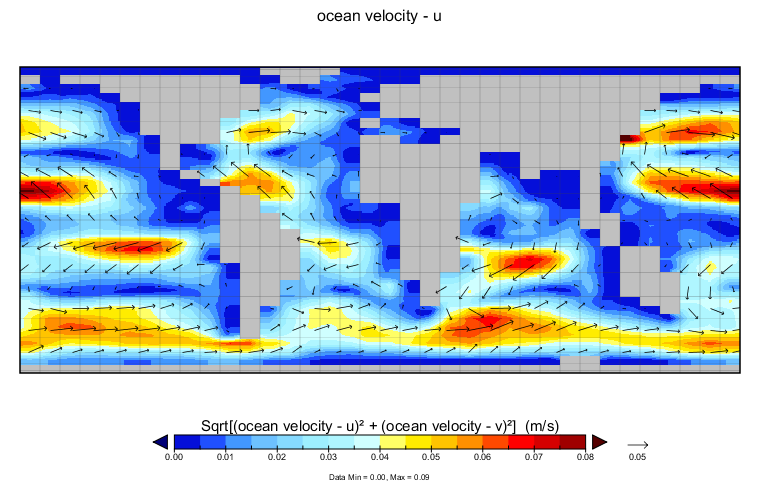
\includegraphics[width=0.6\textwidth]{ch3-currents1.png}\centering
\vspace{-0mm}
\caption{Example plot of (normal/default modern) ocean current fields (3D netCDF file). Again scaling has been set manually to create an easy-to-interpret axis scale. On the left is the surface field, and on the right an intermediate depth (illustrating what approximates the Deep Western Boundary current in the model in the Atlantic).}
\label{fig:ch3-currents1}
\end{figure}

%------------------------------------------------
\vspace{1mm}
\noindent\rule{4cm}{0.5pt}
\vspace{2mm}
%------------------------------------------------

\noindent The second approach is to visualize the large-scale ocean transport in terms of the meridional overturning circulation ('stream-function') (e.g. see background literature).

Two example plots (using \textbf{Panoply}) are shown in Figure \ref{fig:ch3-amoc1} for the Atlantic basin, and Figure \ref{fig:ch3-amoc2} for the Pacific. In the In the 2D \textbf{netCDF} file, relevant fields (netCDF variables)\footnote{Note that these fields are only meaningful for the modern arrangement of the continents and a continuous separation of the Atlantic from the Pacific from high northern latitudes down to the tip of South America. Different (e.g. paleo) arrangements of the continents may not have recognisable (or definable) Atlantic and/or Pacific basins and it may only be possible to define and visualize the global meridional overturning circulation -- variable: \textsf{\footnotesize phys\_opsi}.} are:
\begin{itemize}[noitemsep]
\setlength{\itemindent}{.0in}
\item [] \textsf{\footnotesize phys\_opsia} == global overturning stream-function
\item [] \textsf{\footnotesize phys\_opsip} == overturning in the Atlantic
\end{itemize}

\begin{figure}
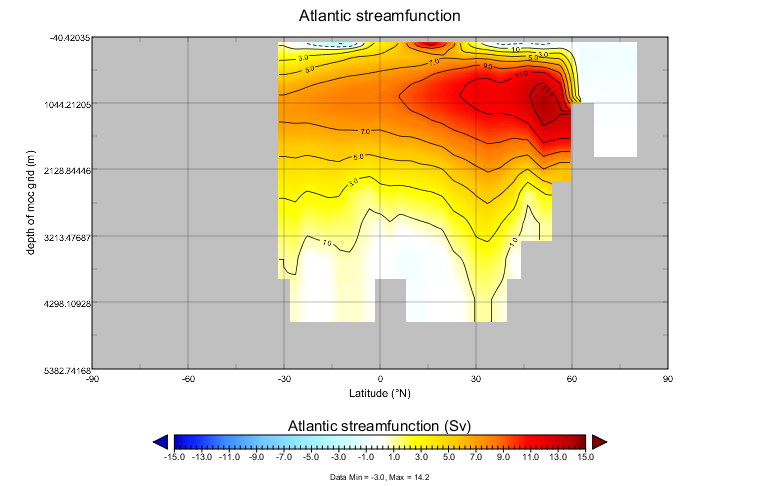
\includegraphics[width=0.6\textwidth]{ch3-amoc1.png}\centering
\vspace{-0mm}
\caption{Example plot of (normal/default modern) overturning stream-function (2D \textbf{netCDF} file). (e.g., for Atlantic: \textbf{netCDF} parameter name: \texttt{phys\_opsia}, long-name: Atlantic stream-function). Note that auto-scaling has been turned off and the min and max plotting limits set manually. By convention, stream-functions are plotted with their scale symmetrical around zero, giving red and ‘warm’ colors for positive value and clockwise overturning, and blues and ‘cold’ colors for negative values and anti-clockwise overturning. (The plot has been tart-ed up by overlaying solid contours plus contour labels.) It may be necessary in \textbf{Panoply} to re-orient (invert) the vertical grid.}
\label{fig:ch3-amoc1}
\end{figure}

\begin{figure}
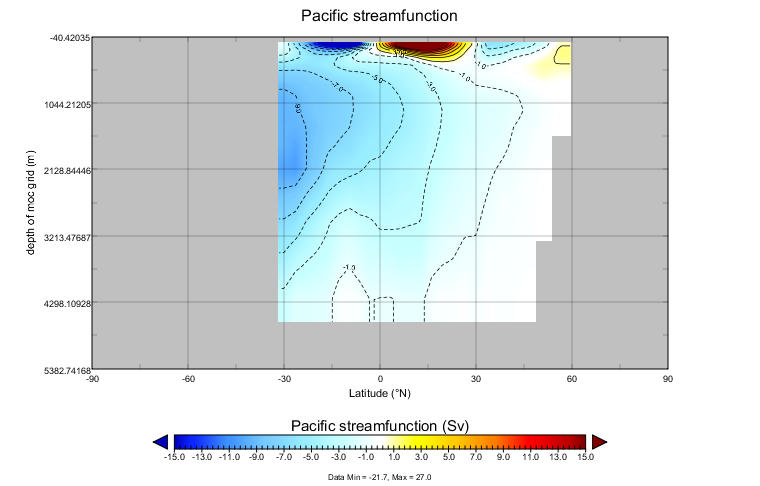
\includegraphics[width=0.6\textwidth]{ch3-amoc2.png}\centering
\vspace{-0mm}
\caption{Pacific meridional overturning circulation (PMOC).}
\label{fig:ch3-amoc2}
\end{figure}

%------------------------------------------------
\newpage
%------------------------------------------------

\section{Tracing ocean circulation}

The ocean biogeochemistry module (\textbf{BIOGEM}) in \textbf{cookie} provides a framework for applying time- and spatially-variable ‘forcings’ of the Earth system\footnote{Refer to the '\textit{force the system}' \textsf{HOW-TO} in the cookie manual for further details on \textit{forcings}.} – fluxes or 'restored-to' boundary conditions that can be prescribed for any gas, dissolved substance (including temperature and salinity), or particulate matter. Examples include freshwater input (== a negative salinity flux forcing) of the North Atlantic to alter ocean circulation, fossil fuel \(CO_{2}\) emissions to the atmosphere (== a \(CO_{2}\) gas flux forcing), or aeolian iron supply to the surface ocean (a 2-D dust flux forcing).

\vspace{1mm}
For example: view the \textit{user-config} file: \textsf{\footnotesize LAB.2.2.colortracer} – you will see the following lines (under the heading: ‘\texttt{\# --- FORCINGS ---}’)

\vspace{-2mm}\small
\begin{verbatim}
bg_par_forcing_name="pyyyyz_Fblue"
bg_par_force_point_i=22
bg_par_force_point_j=33
bg_par_force_point_k=8
bg_par_ocn_force_scale_val_49=1.0E12
\end{verbatim}
\normalsize\vspace{-2mm}

The first line points \textbf{cookie} to a directory located in \textsf{\footnotesize cgenie.cookie/genie-forcings} that contains a set of files that define what geochemical property is going to be altered plus information about how the magnitude of the forcing changes with time.

There are then three lines (\texttt{bg\_par\_force\_point\_i=20}, ...) that specify the location in the ocean of the geochemical forcing that is going to be applied. The point sources are specified in (i,j,k) coordinates, which in this case is (22,33,08). For the ocean model resolution we are using, the grid is 36x36x16, and in which: longitude (i) is counted from left-to-right (1 to 36); latitude (j) is counted from bottom-to-top (1 to 36); level depth (k) is counted from downwards top-to-bottom (16 down to 1). Thus, (22,33,08) is a release of tracer in the North Atlantic, a little south of Greenland, and intermediate depth (level = 8 out of 16). Refer to the Figures for how the horizontal (Figure \ref{fig:ch3-ijgrid}) and vertical (Figure \ref{fig:ch3-kgrid}) grid is specified.

Finally, there is a scaling parameter (\texttt{bg\_par\_ocn\_force\_scale\_val\_49}) which modifies the magnitude of the flux to be applied\footnote{Flux \textit{forcings} in \textbf{cookie} are in units of \(mol yr^{-1}\) per model grid point.} -- the default value in the forcing definition itself is just \(1.0 mol yr^{-1}\).

%------------------------------------------------
\newpage 
%------------------------------------------------

%
\begin{figure}
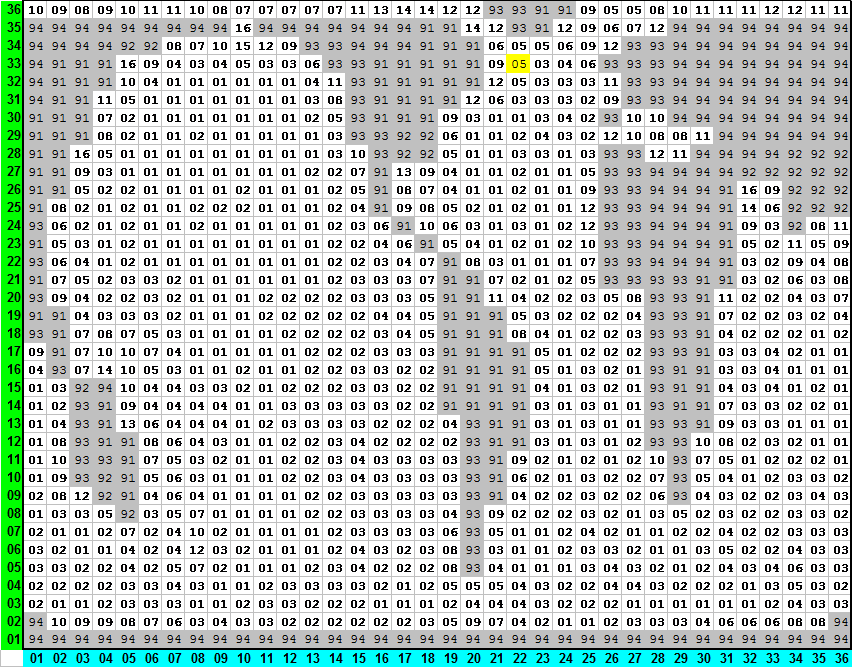
\includegraphics[width=0.8\textwidth]{ch3-ijgrid.png}\centering
\vspace{-0mm}
\caption{
\textbf{The  cookie grid for a modern \(36\times36\) ‘p\_worjh2’ configuration.} Light blue numbers are the ‘i’ co-ordinates. Green numbers are the ‘j’ co-ordinates.
The depth of the ocean at any location is indicated by its ‘k’ value – a number between 1 and 16, with 16 being the surface layer of the ocean, and 1 the maximum possible depth anywhere.
Numbers > 90 (91, 92, 93, 94) and shaded grey are land (and specify the direction of run-off).
Location (22,33,08) is highlighted in yellow.
The longitude of the western edge of this particular modern ocean grid is at 260$^{\circ}$W, and the increments are 10$^{\circ}$.
}
\label{fig:ch3-ijgrid}
\end{figure}

\begin{figure}
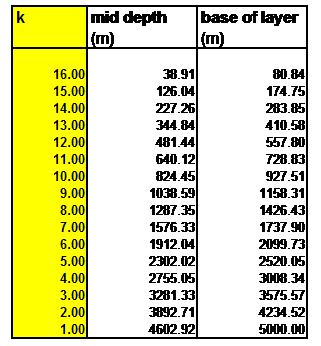
\includegraphics[width=0.4\textwidth]{ch3-kgrid.png}\centering
\vspace{-0mm}
\caption{\textbf{The cookie ocean vertical level definitions for a modern 16-level ocean grid.}}
\label{fig:ch3-kgrid}
\end{figure}

\noindent You are going to run a brief experiment in which you will be injecting a conservative ‘dye’ tracer into the ocean. The \textbf{BIOGEM} module has two tracers that can be defined for this purpose – ‘blue’ and ‘red’ -- you will be using the \uline{blue} one here. You can control the flux of blue dye by opening the \textit{user-config} file: \textsf{\footnotesize LAB.2.2.colortracer} and editing the flux scaling parameter:

\vspace{-2mm}\small\begin{verbatim}
bg_par_ocn_force_scale_val_49=1.0E12
\end{verbatim}\normalsize\vspace{-2mm}

\vspace{1mm}
The \textit{base-config} you will be using is different from previously: \textsf{\footnotesize cookie.C.p\_worjh2.rb} – this specifies a 16 vertical levels ocean and also includes seasonality of solar insolation.\footnote{Note that because the \textit{base-config} is different from that used in the previous chapter, you need to force a re-compile of the model code before any experiments can be submitted as cluster jobs. The easiest way to do this is to run an experiment interactively at the command line.}

%------------------------------------------------
\vspace{1mm}\noindent\rule{4cm}{0.5pt}\vspace{2mm}
%------------------------------------------------

%------------------------------------------------
\newpage 
%------------------------------------------------

\noindent Run the model for … whatever, 20 years will do. Use the \textit{re-start} experiment that you have just downloaded to start from:

\vspace{-2mm}\small\begin{verbatim}
$ ./runcookie.sh cookie.C.p_worjh2.rb LABS LAB.2.2.colortracer 20 
   cookie.C.p_worjh2.rb.SPIN
\end{verbatim}\normalsize\vspace{-2mm}

View the results – for instance how the blue tracer distribution evolves with time – in the \textit{time-slice} files (full ocean/atmosphere) properties saved in the \textbf{netCDF} format (\texttt{.nc}) files). You can follow the progress of the dye (and hence diagnose the properties of ocean circulation in the model) by plotting vertical and/or horizontal slices that go through (or near) the cell location in which you inject the dye tracer in the 3D \textbf{netCDF} file. Note that \textbf{Panoply} appears to ‘count’ the ocean layers in the opposite direction to the way in which the ocean model is actually counting them – the correct definition is with ‘1’ being very deepest level possible (and as displayed in the figure) and '16' is the surface.

You can also view the tracer distributions in terms of a water-column integrated tracer inventory (\textbf{netCDF} variable name: \textsf{\footnotesize ocn\_int\_colb}; long name: \textsf{\footnotesize colb water-column integrated tracer inventory}) in the 2D \textbf{netCDF} output. (See: \textit{Sabine et al.} [2004] for the use of water column integrals in the context of the distribution of anthropogenic \(CO_{2}\) uptake and storage.) Changes in tracer inventory with time can be tracked in the time-series file: \textsf{\footnotesize biogem\_series\_ocn\_colb.res}

Spend a little while altering the flux (\texttt{\small bg\_par\_ocn\_force\_scale\_val\_49}) and/or location
\\(\texttt{\small bg\_par\_force\_point\_i}, \texttt{\small bg\_par\_force\_point\_j, bg\_par\_force\_point\_k}) of tracer input. Overall -- note how you can use numerical ‘tracers’ to help diagnose (and better understand) the circulation of the ocean.

\large\uline{Ignore the 'red' tracer for now ... we'll look at that shortly.}\normalsize

%------------------------------------------------
\vspace{1mm}\noindent\rule{4cm}{0.5pt}\vspace{2mm}
%------------------------------------------------

%------------------------------------------------
\newpage 
%------------------------------------------------
%
\noindent When you add the numerical dye, particularly early on in the experiment, you may see a 'front' of \uline{negative} tracer concentrations leading the (positive) tracer as it spreads. DON'T PANIC!

The model is ... a model (of the numerical flavor) and not an exact analytical solution. So errors in how it solves ocean transport are to be expected.

Moreover, by default the ocean circulation model employs an isopycnal/diapycnal mixing scheme. This can lead to unwanted negative tracer values when sharp horizontal (or vertical) transitions in concentration occur. (In this example, e.g. by injection dye at a point location into a surrounding ocean of initially zero concentration.)

You can change to a simpler horizontal/vertical (.false.) mixing scheme by adding to the \textit{user-config} file:

\vspace{-2mm}\small\begin{verbatim}
# turn OFF (=.false.) isopycnal/diapycnal mixing
go_diso=.false.
\end{verbatim}\normalsize\vspace{-2mm}

If you try this, you should (hopefully) find much less (or no) negative tracer concentrations occur. However, also note that by changing the physics of ocean mixing, you also slightly alter the large-scale circulation of the ocean (and e.g. the AMOC might change slightly in strength).\footnote{You might contrast the overturning stream-functions for experiments run both with and without horizontal/vertical mixing.} 

%------------------------------------------------
\vspace{1mm}\noindent\rule{4cm}{0.5pt}\vspace{2mm}
%------------------------------------------------

\noindent Lastly, an interesting (honest!) and illustrative exercise is to use the dye tracer to pick out the path taken by Mediterranean Intermediate Water. Despite the low resolution of the \textbf{cookie} ocean circulation model component and the highly restricted representation of the Mediterranean, the model does project a salty Mediterranean as a consequence of  P-E across this basin (and its catchments) being negative and this higher density water makes its way out in the subsurface into the Atlantic.

To do this -- simply specify a dye injection somewhere in the Mediterranean (be careful with the restricted depth of the Mediterranean – if you inject too deeply (into the crust!) then you will not see anything (refer to the figure for the depth level (k) number of the maximum depth of the water column in each location), and it is better to inject it relatively close to the opening of the gateway (try some different locations and see which ones produce a reasonably instructive tracing of Mediterranean outflow). Run for e.g., 20 or 50 years (from the provided spin-up). Then:

\vspace{1mm}
\begin{enumerate}[noitemsep]
\vspace{1mm}
\item View the dye-tagged plume of Mediterranean Intermediate Water by plotting a lat-lon slice (from the 3D \textbf{netCDF} file). This will give you the depth of the plume. How does this compare with salinity observations (salinity observations and appropriate global data-sets can be found on the web with a little patience)? You can also view the water-column integrated distribution (2D \textbf{netCDF}).
\vspace{1mm}
\item Try viewing the plume via a lat-depth slice. Refer to the figure to determine the ‘i’ value up the Atlantic that will just graze the edge of what passes for Spain at this low model resolution. Which direction does it head after exiting the Mediterranean? Is this ‘realistic’?
\end{enumerate}
\vspace{1mm}

%------------------------------------------------
\newpage
%------------------------------------------------

\section{Tracing ocean ... ventilation}

Yet another way to think about global ocean circulation is through considering the connection (rate of mass exchange) between surface and deep ocean -- 'ventilation'.

\textbf{cookie} has the capability to employ/simulate a ventilation age tracer\footnote{Under the '\textit{screw with and/or diagnose the climate system}' HOW-DO -- see '\textit{Add a water mass age tracer}' (and the 'easy'/automatic method described towards the end of that section).} -- a numerical tracer carried in the ocean circulation model that tracks the time since a parcel of water last 'saw' the surface. The older the 'age' of the parcel of water, the longer the time since it last saw the surface.

We can use the second numerical tracer (red') to keep track of age, but rather than apply a flux forcing to the surface, we let the model automatically restore the tracer value at the surface to zero and everywhere else (in the ocean interior) increase the age each time-step (by the duration of the time-step) such that a parcel of water away from the surface ages by 1 year, each year.

The \textit{base-config}, and \textit{restart}, provided for the ('blue') circulation tracing, already has the ('red') age tracer included and activated. As a result, all of your experiments on ocean circulation which you have conducted so far already have simulated ocean ventilation age and you do not need to run a new experiment (unless you want to!).

%------------------------------------------------
\vspace{1mm}\noindent\rule{4cm}{0.5pt}\vspace{2mm}
%------------------------------------------------

\noindent In the 3D netCDF output file -- \textsf{\footnotesize misc\_col\_Dage} is the output variable that is the calculated ventilation age.

Explore the distribution of water mass age and think about the physical ocean circulations reasons for this. Are all the modelled distributions reasonable? Are there indicators of facets of the simulated circulation that are not particularly realistic? Try plotting both lon-lat and lat-depth slices through the ocean. How does the distribution of water mass age relate to the overturning stream-function for Atlantic or Pacific basins (more on this in the next Section)?

%------------------------------------------------
\newpage
%------------------------------------------------

\section{Poking the climate beast}

Instead of adding a dye tracer, you could add fresh water to the ocean surface to assess the sensitivity of the Atlantic Meridional Overturning Circulation (AMOC) to collapse, in a classic ‘hosing’ experiment.

The \textit{user-config} file for this is called: \textsf{\footnotesize LAB.2.4.hosing}. The default (i,j) location of the flux input is the same (as the dye tracer), but now the injection at the surface (level: k=16). Note that the forcing of the salinity tracer is negative (freshwater = negative salinity compared to sea-water)!

To orientate you in freshwater forcing space: \texttt{bg\_par\_ocn\_force\_scale\_val\_2=-2.0E17} should be sufficient to make ‘stuff happen’ and quickly. BUT, this is a pretty extreme flux (see overleaf for a rough conversion between salinity forcing units (mol yr$^{-1}$) and fresh water flux (in m$^{3}$ s$^{-1}$ or Sv). Much more than this and the model may crash or at the very least, you’ll be left with a large freshwater pond in the North Atlantic … (see later for some exciting discussion on units!)

\vspace{1mm}
To run the model for e.g., 20 years using the same restart:

\vspace{-2mm}\small\begin{verbatim}
$ ./runcookie.sh cookie.C.p_worjh2.rb LABS LAB.2.4.hosing 20 
   cookie.C.p_worjh2.rb.SPIN
\end{verbatim}\normalsize\vspace{-2mm}

\noindent 20 years should be long enough to see a collapse start to occur, but you might want to run the model for longer (and it can be submitted as a job, of course). Running for longer will also allow you to have a smaller, less extreme (and maybe more realistic) freshwater input flux.

Make sure that you run a \uline{control} experiment -- an experiment of the same duration of your hosing experiments, but with a zero freshwater flux. The impact of freshwater input, is the difference, at the same model year, between the perturbation experiment and the control. (You only ever need need to run one control, regardless of how many different freshwater flux perturbation experiments  you run.) 

Note that as the model is running rather s l o w e r than in the snowball configuration, you might want to think carefully of making use of cluster queuing possibilities (i.e., running multiple experiments at once in the background).

%------------------------------------------------
\vspace{1mm}\noindent\rule{4cm}{0.5pt}\vspace{2mm}
%------------------------------------------------

\noindent The most obvious property of the Earth system to follow is the Atlantic overturning strength (\textsf{\footnotesize biogem\_series\_misc\_opsi.res}). The AMOC stream-function (in \textsf{\footnotesize fields\_biogem\_2d.nc} 2-D time-slice \textbf{netCDF} results file, field: \textsf{\footnotesize phys\_opsia}) is also illustrative. You can also try and identify the salinity anomaly (see below) due to freshwater input in the 3D salinity tracer field.

There are also important (but not necessarily painfully exciting) impacts on surface air temperatures and maybe sea-ice extent (in \texttt{fields\_biogem\_2d.nc)} (but see below for a better way to visualize these changes). Note the importance (sort of) of the AMOC in transporting heat to the N Atlantic region (the film the Day After Tomorrow was not entirely inaccurate in this particular respect). Be aware of the possibility of climate impacts far from the location of fresh water forcing. Look out for any significant-looking impacts on sea-ice extent, etc.

You might also plot current velocity fields and visualize how these change in response to the fresh water forcing.

Lastly, if you ran much longer than 20 years, you might start to see impacts on the ocean ventilation age.

%------------------------------------------------
\vspace{1mm}\noindent\rule{4cm}{0.5pt}\vspace{2mm}
%------------------------------------------------

%------------------------------------------------
\newpage
%------------------------------------------------

\noindent To more easily assess some of these impacts (and for other sorts of analysis) it is possible to create an \uline{anomaly (difference) map} in \textbf{Panoply}:

\vspace{1mm}
\begin{enumerate}[noitemsep]
\vspace{1mm}
\item  First open a dataset, e.g., \textsf{\footnotesize atm\_temp} (surface air temperature) in the 2D \textbf{netCDF} file. You can either double-click the variable name, or, with the variable name highlighted, click the ‘Create Plot’ icon.
\vspace{1mm}
\item Now, with the \textsf{\footnotesize atm\_temp} still selected (and the first plot window still open), click on the ‘Combine Plot’ icon. A dialogue box will appear and ask you to select a plot to combine the new one with. Make sure the name of your first plot window is selected/highlighted. Click ‘Combine’. OR, simply drag a second dataset into the plot window of the first dataset.
\vspace{1mm}
\item You now have a plot window that by default it is showing you the difference between two identical (in time) slices. The two different slices are labeled Array 1 (LH side) and Array 2 (RH side).
\end{enumerate}
\vspace{1mm}

Keep one array (Array 1) fixed to the initial (year 1 (centered on 0.5)) and vary the year in the second array (Array 2). Note that you can select in Panoply whether Array 1 – Array 2 is plotted, or Array 2 – Array 1, or various proportional or relative differences.

Note that you can switch off the auto-scaling feature (Always fit to data) and center the scale so that no change is white, with positive deviations = red and negative = blue by clicking on Center on 0 (an often used convention in climate field plotting).

%------------------------------------------------
\vspace{1mm}\noindent\rule{4cm}{0.5pt}\vspace{2mm}
%------------------------------------------------

\noindent Finally, a brief note on units ... the freshwater forcing is implemented as negative salinity, just to really screw with your mind. The generic internal \textbf{cookie} model units for the forcing end up as \(PSU kg^{-1} yr^{-1}\). Which sort of does not make much sense ...

Start, by thinking of a value of \texttt{bg\_par\_ocn\_force\_scale\_val\_2} of \(-34.9\) as equivalent to taking all the salt out of \(1 kg\) of freshwater (since the mean global salinity is \(34.9 PSU\)). Or equivalently, since the ocean volume is fixed, an applied forcing value of \(-34.9\) is equivalent to adding \(1 kg\) of freshwater to a (surface) box. So, a value of \texttt{bg\_par\_ocn\_force\_scale\_val\_2} of \(-3.49\times10^{4}\) (\(-3.49E04)\) would be a flux of \(1 m^{3} yr^{-1}\) (\(1000 kg m^{-3}\)) of freshwater.

So, in the example earlier (\texttt{bg\_par\_ocn\_force\_scale\_val\_2=-1.0E18}), the freshwater flux is \(1.0\times10^{18}/3.49\times10^{4} = 2.8653\times10^{13} m^{3} yr^{-1}\).

The literature invariably gives freshwater fluxes in units of \(Sv\) (\(10^{6} m^{3} s^{-1}\)). So in the example, the freshwater flux is: \(9.0797\times10^{5} m^{3} s^{-1}\) (\(365.25\times24\times3600 = 31557600 s yr^{-1}\)). Or \(0.9 Sv\).

Or or ... \(1.0 Sv\) is equivalent to a model (\texttt{bg\_par\_ocn\_force\_scale\_val\_2}) total forcing flux of \(-1.0E18/0.90797 = -1.1E18\)

Read the literature … but generally, fluxes of ca. \(0.05 Sv\) and larger (and to quite specific places) are applied in models to induce an AMOC collapse.

%------------------------------------------------
\newpage
%------------------------------------------------

\section{Further ideas}

%------------------------------------------------

\subsection{Assessing the spatial sensitivity of deep-water formation to shutdown}

What is the largest freshwater flux that can be sustained without ‘collapsing’ the AMOC? Is there a ‘threshold’ (‘tipping point’) of freshwater input, beyond which the AMOC rapidly decreases in strength? For this -- you would run (submit to the cluster) a series of experiments, each with different (increasing) values for the fresh water flux. Remember to include an experiment with zero freshwater flux to act as a 'control'.

Is the precise location of the freshwater input important (i.e., try tipping it in somewhere else)? For this -- you could piece-meal run an experiment, analyse the results, then choose a new location to input the freshwater, or, come up with a systematic search pattern of freshwater input patterns.  

Outside of the North Atlantic, are any other  regions (of deep water formation) sensitive to freshwater perturbation and what are the consequences (could it happen in the future)?

%------------------------------------------------

\subsection{Forcing stronger deep-water formation (‘anti-hosing’ investigations)}

There are questions concerning past changes in the AMOC as to whether it is ‘pushed’ or ‘pulled’. i.e., if the AMOC shoals in depth and/or weakens, is it because its production has weakened, or as Antarctic Bottom water (AABW) strengthened and ‘pushed’ it out of the way (to shallower depths)?

What you might try then is to inject salt in the Southern Ocean as opposed to fresh water in the North Atlantic. All you need do is pick an appropriate grid point (this is worth thinking about carefully and maybe testing different locations) and rather than giving the parameter \texttt{bg\_par\_ocn\_force\_scale\_val\_2} a negative value, you give it a positive one. (Start by trying similar magnitudes of value as before and see what happens.)

\textbf{Is the AMOC (for the same magnitude of forcing) more sensitive to being ‘pushed’ or ‘pulled’?} (Obviously the answer will  depend on where the perturbations are being applied.)

%------------------------------------------------

\subsection{Response to transient warming}

A current concern regarding anthropogenic climate change is the ocean circulation (and marine ecological and biogeochemical) response to a strong warming of the surface, as rapid surface warming is assumed (and demonstrated in models) to result in surface stratification of the ocean, likely restricting the nutrient supply to phytoplankton and reducing ventilation of the ocean interior with dissolved oxygen.

You can explore the transient response of ocean circulation to warming by simply adjusting the radiative forcing parameter as per used in the snowball Earth experiments: \texttt{ea\_radfor\_scl\_co2}. By default in the modern continental configuration, this has a value of 1.0, corresponding to 278 ppm atmospheric \(CO_{2}\). A value of 2.0 would reflect warming equivalent to 556 ppm \(CO_{2}\). And 3.0 more like an end-of-the-century warming. Note that you are applying the warming instantaneously by manipulating the climate system in this way and hence the changes will be more extreme than those occurring over the time-scale of this century. Also note that a cooling (a radiative scaling small er than $1.0$) could be applied instead.

Potentially interesting properties of the Earth system to look at include sea-ice extent and AMOC strength (in the ASCII time-series files), and the overturning stream-function and sea-ice extent in the 2-D \textbf{netCDF} output. It is also possible to fresh water force the model with an age tracer and hence make projections of how patterns of ventilation age change with transient warming.

Overall, try and answer the question: \textbf{How much radiative forcing is required to collapse the AMOC? What atmospheric \(CO_{2}\) value does this approximately correspond to?}

%------------------------------------------------

\subsection{Regional hosing}

\noindent It is also possible to apply freshwater fluxes in a specific pattern/region, rather than just at a single location.

%----------------------------------------------------------------------------------------
%----------------------------------------------------------------------------------------
%----------------------------------------------------------------------------------------
%       CHAPTER 3
%----------------------------------------------------------------------------------------

\cleardoublepage

\chapterimage{middle_earth.png} % Chapter heading image

\chapter{Ocean circulation II (fake worlds)}\label{ch:ocean-circulation-II}

\hfill \break

%------------------------------------------------
\newpage
%------------------------------------------------

\section{(none)}

%----------------------------------------------------------------------------------------
%----------------------------------------------------------------------------------------
%----------------------------------------------------------------------------------------
%       CHAPTER 4
%----------------------------------------------------------------------------------------

\cleardoublepage

\chapterimage{Hurricane-Irma.png} % Chapter heading image

\chapter{Atmospheric dynamics}\label{ch:atmospheric-dynamics}

\hfill \break

%------------------------------------------------
\newpage
%------------------------------------------------

\section{(none)}

%----------------------------------------------------------------------------------------
%----------------------------------------------------------------------------------------
%----------------------------------------------------------------------------------------
%       CHAPTER 5
%----------------------------------------------------------------------------------------

\cleardoublepage

\chapterimage{oceanacidification.png} % Chapter heading image

\chapter{Fossil fuel CO$_{2}$ and 'ocean acidification'}

\hfill \break

%------------------------------------------------
\newpage
%------------------------------------------------

\section{(none)}

%----------------------------------------------------------------------------------------
%----------------------------------------------------------------------------------------
%----------------------------------------------------------------------------------------
%       CHAPTER 6
%----------------------------------------------------------------------------------------

\cleardoublepage

\chapterimage{oceanacidification.png} % Chapter heading image

\chapter{Fossil fuel CO$_{2}$ and 'ocean acidification'}

\hfill \break

%------------------------------------------------
\newpage
%------------------------------------------------

\section{(none)}

%----------------------------------------------------------------------------------------
%----------------------------------------------------------------------------------------
%----------------------------------------------------------------------------------------
%       CHAPTER 7
%----------------------------------------------------------------------------------------

\cleardoublepage

\chapterimage{chx-biogeo.png} % Chapter heading image

\chapter{Ocean biogeochemical cycles}\label{ch:ocean=biogeochem}

\hfill \break

%------------------------------------------------
\newpage
%------------------------------------------------

\section{(none)}

%----------------------------------------------------------------------------------------
%----------------------------------------------------------------------------------------
%----------------------------------------------------------------------------------------
%       CHAPTER 8
%----------------------------------------------------------------------------------------

\cleardoublepage

\chapterimage{origin.jpg} % Chapter heading image

\chapter{The geological cycle of carbon}\label{ch:geological-carbon}

\hfill \break

%------------------------------------------------
\newpage
%------------------------------------------------

\section{(none)}

%----------------------------------------------------------------------------------------
%----------------------------------------------------------------------------------------
%----------------------------------------------------------------------------------------
%       CHAPTER 09
%----------------------------------------------------------------------------------------

\cleardoublepage

%\chapterimage{xxx} % Chapter heading image

\chapter{xxx}\label{ch:09}

\hfill \break

%------------------------------------------------
\newpage
%------------------------------------------------

\section{(none)}

%----------------------------------------------------------------------------------------
%----------------------------------------------------------------------------------------
%----------------------------------------------------------------------------------------
%       CHAPTER 10
%----------------------------------------------------------------------------------------

\cleardoublepage

%\chapterimage{xxx} % Chapter heading image

\chapter{xxx}\label{ch:10}

\hfill \break

%------------------------------------------------
\newpage
%------------------------------------------------

\section{(none)}

%----------------------------------------------------------------------------------------
%----------------------------------------------------------------------------------------
%----------------------------------------------------------------------------------------
%       CHAPTER 11
%----------------------------------------------------------------------------------------

\cleardoublepage

\chapterimage{13750210193_e161c3ede1_b.jpg} % Chapter heading image

\chapter{Proxies and Reconstructing the Past}\label{ch:proxies}

\hfill \break

%------------------------------------------------
\newpage
%------------------------------------------------

\section{(none)}

%----------------------------------------------------------------------------------------
%----------------------------------------------------------------------------------------
%----------------------------------------------------------------------------------------
%       CHAPTER 12
%----------------------------------------------------------------------------------------

\cleardoublepage

%\chapterimage{xxx} % Chapter heading image

\chapter{xxx}\label{ch:12}

\hfill \break

%------------------------------------------------
\newpage
%------------------------------------------------

\section{(none)}

%----------------------------------------------------------------------------------------
%----------------------------------------------------------------------------------------
%----------------------------------------------------------------------------------------
%       CHAPTER 13
%----------------------------------------------------------------------------------------

\cleardoublepage

%\chapterimage{xxx} % Chapter heading image

\chapter{xxx}\label{ch:13}

\hfill \break

%------------------------------------------------
\newpage
%------------------------------------------------

\section{(none)}

%----------------------------------------------------------------------------------------
%----------------------------------------------------------------------------------------
%----------------------------------------------------------------------------------------
%       CHAPTER 14
%----------------------------------------------------------------------------------------

\cleardoublepage

%\chapterimage{xxx} % Chapter heading image

\chapter{xxx}\label{ch:14}

\hfill \break

%------------------------------------------------
\newpage
%------------------------------------------------

\section{(none)}

%----------------------------------------------------------------------------------------
%----------------------------------------------------------------------------------------
%----------------------------------------------------------------------------------------
%       CHAPTER 15
%----------------------------------------------------------------------------------------

\cleardoublepage

\chapterimage{chx-plotting.png} % Chapter heading image

\chapter{muffinplot}\label{ch:muffinplot}

\hfill \break

%------------------------------------------------
\newpage
%------------------------------------------------

\section{(none)}

%----------------------------------------------------------------------------------------
%----------------------------------------------------------------------------------------
%----------------------------------------------------------------------------------------
%       CHAPTER 16
%----------------------------------------------------------------------------------------

\cleardoublepage

\chapterimage{big-data.jpg} % Chapter heading image

\chapter{muffindata}\label{ch:muffindata}

\hfill \break

%------------------------------------------------
\newpage
%------------------------------------------------

\section{(none)}

%----------------------------------------------------------------------------------------
%----------------------------------------------------------------------------------------
%----------------------------------------------------------------------------------------
%       CHAPTER 17
%----------------------------------------------------------------------------------------

\cleardoublepage

%\chapterimage{xxx} % Chapter heading image

\chapter{xxx}\label{ch:17}

\hfill \break

%------------------------------------------------
\newpage
%------------------------------------------------

\section{(none)}

%----------------------------------------------------------------------------------------
%----------------------------------------------------------------------------------------
%----------------------------------------------------------------------------------------
%       CHAPTER 18
%----------------------------------------------------------------------------------------

\cleardoublepage

%\chapterimage{xxx} % Chapter heading image

\chapter{xxx}\label{ch:18}

\hfill \break

%------------------------------------------------
\newpage
%------------------------------------------------

\section{(none)}

%----------------------------------------------------------------------------------------
%----------------------------------------------------------------------------------------
%----------------------------------------------------------------------------------------
%       CHAPTER 19
%----------------------------------------------------------------------------------------

\cleardoublepage

\chapterimage{ch-howto.png} % Chapter heading image

\chapter{HOW-TO (technical)}\label{ch:how-to-technical}

\hfill \break

%------------------------------------------------
\newpage
%------------------------------------------------

\section{(none)}

%----------------------------------------------------------------------------------------
%----------------------------------------------------------------------------------------
%----------------------------------------------------------------------------------------
%       CHAPTER 20
%----------------------------------------------------------------------------------------

\cleardoublepage

\chapterimage{ch-howto.png} % Chapter heading image

\chapter{HOW-TO (experiment)}\label{ch:how-to-experiment}

\hfill \break

%------------------------------------------------
\newpage
%------------------------------------------------

\section{(none)}

%----------------------------------------------------------------------------------------
%----------------------------------------------------------------------------------------
%----------------------------------------------------------------------------------------
%       CHAPTER 21
%----------------------------------------------------------------------------------------

\cleardoublepage

\chapterimage{muffin_planet.jpg} % Chapter heading image

\chapter{cookie Development}\label{ch:model-code}

\hfill \break

%------------------------------------------------
\newpage
%------------------------------------------------

\section{(none)}

%----------------------------------------------------------------------------------------
%----------------------------------------------------------------------------------------

%----------------------------------------------------------------------------------------
%----------------------------------------------------------------------------------------

\backmatter

%----------------------------------------------------------------------------------------
%       INDEX
%----------------------------------------------------------------------------------------

%\cleardoublepage
%\phantomsection
%\setlength{\columnsep}{0.75cm}
%\addcontentsline{toc}{chapter}{\textcolor{ocre}{Index}}
%\printindex

%----------------------------------------------------------------------------------------

\end{document}

%----------------------------------------------------------------------------------------
%----------------------------------------------------------------------------------------
%----------------------------------------------------------------------------------------